%======================================================================
\chapter{Nested Simulation Procedures in Financial Engineering: A Selected Review}\label{chap:project1}
%======================================================================


\section{Introduction}

Nested simulation procedures are commonly used in financial engineering to estimate risk measures for portfolios of complex financial derivatives. 
The term \textit{nested} refers to a nested estimation problem, in which the estimation of the risk measure requires two levels of \gls{mc} simulations.
In a typical nested simulation procedure, an outer-level simulation model generates underlying risk factors, which are referred to as the \textit{outer scenarios}.
For each outer scenario, an inner-level simulation model generates scenario-wise samples of the portfolio losses, which are referred to as the \textit{inner replications}.

The nested simulation procedure is computationally expensive due to its nested structure. 
Given a fixed computational budget, the nested simulation procedure should balance the number of outer scenarios and the number of inner replications to maximize computational efficiency.
\cite{gordy2010nested} first analyzed and proposed an optimal budget allocation for a standard nested simulation procedure.
The term \textit{standard} refers to using a standard \gls{mc} estimator, the sample mean of the inner replications to estimate a scenario-wise portfolio loss for an outer scenario.
\cite{gordy2010nested} investigate an optimal budget allocation for a standard nested simulation procedure with respect to the \gls{mse} of the estimated risk measure.

The standard nested simulation procedure is computationally expensive with a wasteful use of the simulation budget, as only the inner replications from the same outer scenario are used in estimating the scenario-wise portfolio loss for that outer scenario.
Subsequent research efforts have been made to improve the efficiency of nested simulation procedures by using inner replications from other outer scenarios.
This is referred to as pooling.
Different methods pool inner replications differently, using either a trained supervised learning metamodel or predefined likelihood ratio weights.
\cite{broadie2015risk} propose a regression-based nested simulation procedure, which uses a trained regression metamodel to estimate the scenario-wise portfolio loss for an outer scenario by pooling the inner replications from all outer scenarios.
For certain risk measures,~\cite{broadie2015risk} show that it's optimal to allocate the entire simulation budget to outer-level simulations, keeping only 1 inner replication in each outer scenario.
Similarly,~\cite{hong2017kernel},~\cite{feng2020optimal}, and~\cite{zhang2022sample} use a kernel smoothing model, a likelihood ratio model, and a \gls{krr} model as metamodels to pool the inner replications from all outer scenarios, respectively.
In simulation studies, this approach—using a model of a simulation—is called metamodeling, and such models are termed metamodels~\citep{barton1998simulation}.
Another line of research is a \gls{mlmc} method analyzed in~\cite{giles2019multilevel}, which is a variance reduction technique that uses a hierarchy of approximations to the quantity of interest.

This paper presents a survey study of some popular nested simulation procedures that have both asymptotic convergence analysis and finite-sample performance evaluation.
Many procedures have been proposed in the literature, but they are not directly comparable because they use different assumptions and different numerical examples in their studies.
Within a common analytical framework, we first summarize and compare the asymptotic convergence rates of these procedures.
Their asymptotic convergence results are closely examined for their assumptions that guarantee the convergence.

In terms of finite-sample performance, different studies propose different examples in their numerical experiments, which introduces unfair advantages for certain simulation procedures over others. 
A fair comparison among popular methods is therefore urgently needed in the literature. 
Our numerical experiment in this chapter is the first of its kind to subject all the aforementioned simulation procedures to a fair comparison. 
As a result, extensive numerical experiments are conducted to show, in practical examples, how well the finite-sample performance of a method matches its theoretical convergence behavior. 
Through our numerical examples, we compare the nested simulation procedures for different payoff complexities, problem dimensions, and risk measures. 
This chapter also provides a discussion of the computational complexity of different nested simulation procedures, including additional computational costs for training supervised learning metamodels and pooling inner replications.

The rest of this chapter is organized as follows.
Section~\ref{sec1:problem-formulation} introduces the nested simulation procedure and the standard \gls{mc} estimator.
Section~\ref{sec1:asymptotic-convergence} provides new theoretical results on the convergence of existing nested simulation procedures.
Section~\ref{sec1:convergence-orders} summarizes the asymptotic convergence orders and the critical assumptions of nested simulation procedures in the literature.
Section~\ref{sec1:numerical-experiments} presents the numerical experiments and the comparisons of different nested simulation procedures with respect to different risk measures, problem dimensions, and payoff complexities.
Section~\ref{sec1:computational-complexity} discusses the computational complexity of different nested simulation procedures.
Section~\ref{sec1:conclusion} concludes this chapter.
In appendix, we briefly sketch out connections between two modes of convergence for nested simulation procedures.

\section{Problem Formulation}\label{sec1:problem-formulation}

In a nested estimation problem, we are interested in estimating the quantity 

$$\rho(L) = \rho(L(X)),$$
where $X \in \mathcal{X} \subset \mathbb{R}^d$, and $L = L(X)$ is a random variable whose distribution is characterized by $X$.
$L(X)$ is not subject to direct evaluation, but it is the output of 

$$ L(X) = \mathbb{E}\left[ Y|X=x \right]\vert_{x=X} $$

Some common risk measures are in the nested expectation form as
$$\rho(L) = \mathbb{E}\left[ h(L) \right]$$
where $h: \mathbb{R} \mapsto \mathbb{R}$ is a known nonlinear function. 
The nested expectation form is a general form that covers many risk measures of interest in financial engineering by varying the function $h$.
Common forms of $h$ in the literature include smooth functions, Lipschitz continuous functions, and indicator functions.

\begin{definition}\label{def1:smooth}
    A function $h: \mathbb{R} \mapsto \mathbb{R}$ is smooth if it is continuously differentiable up to the $n$-th order for some $n \in \mathbb{N}$, 
    and its $n$-th and $m$-th derivatives are bounded for some $m \in \mathbb{N}$ and $m < n$.
\end{definition}

A quadratic tracking error with benchmark $b$, where $h(t) = (t - b)^2$, falls into this category.
In the context of nested estimation for smooth $h$, different procedures require different versions of Definition~\ref{def1:smooth} to specify the smoothness for their convergence analysis.
Table~\ref{tab1:smoothness} summarizes the smoothness assumption of $h$ for different nested simulation procedures in the literature.

\begin{table}[ht!]
    \centering
    \begin{tabular}{lcc}
    \toprule
    \textbf{Nested Simulation Procedures} & $n$ & $m$ \\
    \midrule
    Regression & $2$ & not required \\
    Kernel smoothing & $3$ & $2$ \\
    Kernel ridge regression & $2$ & $1$ \\
    Likelihood ratio & $2$ & $1$ \\
    \bottomrule
    \end{tabular}
    \caption{Smoothness assumption of $h$ for different nested simulation procedures}
\label{tab1:smoothness}
\end{table}

The regression-based nested simulation procedure has the least stringent smoothness assumption.
In general, a more complex metamodel requires a higher-order smoothness for $h$ for its convergence analysis.
Despite being more advanced than kernel smoothing, the \gls{krr}-based procedure requires a less stringent smoothness assumption on $h$.
At first sight, it is counterintuitive that a more complex metamodel requires a less stringent smoothness assumption.
This phenomenon is due to the fact that the convergence analysis for the \gls{krr}-based nested simulation procedure is shown in terms of \gls{ae}, a different error metric than \gls{mse}.
In appendix, we include a discussion of the connection between the \gls{mse} and the \gls{ae} of the estimator in the context of nested simulation procedures.
In Table~\ref{tab1:smoothness}, the standard nested simulation procedure is the only procedure without an asymptotic convergence analysis for smooth $h$.
Section~\ref{sec1:sns} fills this gap by providing the asymptotic convergence analysis for the standard nested simulation procedure in terms of \gls{mse}.

\begin{definition}\label{def1:lipschitz}
    A function $h: \mathbb{R} \mapsto \mathbb{R}$ is Lipschitz continuous with a Lipschitz constant $K$ if for all $t_1, t_2 \in \mathbb{R}$, 
    $$|h(t_1) - h(t_2)| \leq K|t_1 - t_2|.$$
\end{definition}

The mean excess loss over a threshold $u$ is defined by setting $h(t) = \max\{t - u, 0\}$, which is a special case of a Lipschitz continuous function.
The regression-based nested simulation procedure is the only procedure that performs a theoretical analysis for Lipschitz continuous $h$.
The other procedures only provide a convergence analysis for the special case of mean excess loss over a threshold $u$.

\begin{definition}\label{def1:indicator}
    A function $h: \mathbb{R} \mapsto \mathbb{R}$ is an indicator function if 
    $$h(t) = \mathbb{I}_{\{t \geq u\}}$$
    for some $u \in \mathbb{R}$.
\end{definition}

The probability of a large loss over a threshold $u$ is obtained by setting $h(t) = \mathbb{I}_{\{t \geq u\}}$.

Other risk measures of interest not in the nested expectation form include \gls{var} and \gls{cvar}~\citep{hardy2022quantitative}. 
The $\alpha$-\gls{var} of $L$ is defined as
\begin{equation}\label{eq1:var}
    \mbox{VaR}_\alpha(L) = q_\alpha = \inf \left\{ q: \Pr(L\leq q) \geq \alpha \right\}.
\end{equation}
    
The $\alpha$-\gls{cvar} of $L$ is defined as
\begin{equation}\label{eq1:cvar}
    \mbox{CVaR}_\alpha(L) =\frac{1}{1-\alpha} \int_{\alpha}^{1} q_v dv. 
\end{equation}

In the literature, \gls{cvar} are also known as Conditional Tail Expectation (CTE), Tail Value-at-Risk (TailVaR), and Expected Shortfall (ES).

The rest of this section reviews the existing nested simulation procedures in the literature.
We unify their notations and provide a comprehensive comparison of how inner replications are generated and pooled for different procedures.

\subsection{The Standard Nested Simulation Procedure}

The standard nested simulation procedure first simulates $M$ independent and identically distributed (i.i.d.) outer scenarios $X_1, \dots, X_M$ from $F_X$, the distribution of $X$.
For each $X_i$, again simulate $Y_{ij}$, $j = 1, \dots, N$ from $F_{Y|X_i}$, the conditional distribution of $Y$ given $X_i$.
Given scenario $i$, the $Y_{ij}$ are conditionally i.i.d.
Let $\Gamma = M \cdot N$ denote the total simulation budget, $f_X(x)$ denote the density of $X$, and $\mathbf{X} = (X_1, \dots, X_M)$ denote the vector of outer scenarios.

The standard nested simulation procedure estimates $L_i = L(X_i)$ with a standard \gls{mc} estimator 
\begin{equation*}
  \hat{L}_{N, i} = \frac{1}{N} \sum_{j=1}^N Y_{ij}, \quad Y_{ij} \sim F_{Y|X_i}.  
\end{equation*}

Let $\hat{L}_{(i)}, \dots, \hat{L}_{(M)}$ be the order statistics of $\hat{L}_{N, 1}, \dots, \hat{L}_{N, M}$. 
The standard nested simulation estimators for different forms of $\rho$ are as follows:

\begin{enumerate}
    \item   Nested expectation form:
            \begin{equation*}
                \hat{\rho}_{M, N} = \frac{1}{M} \sum_{i=1}^M h(\hat{L}_{N, i}) = \frac{1}{M} \sum_{i=1}^M h(\bar{Y}_{N, i}), \quad X_i \sim F_X.
            \end{equation*}
    \item   \gls{var}:
            \begin{equation*}
                \hat{\rho}_{M, N} = \hat{L}_{(\lceil \alpha M \rceil)}.
            \end{equation*}

    \item   \gls{cvar}:
            \begin{equation}\label{eq1:cvar-hat}
                \hat{\rho}_{M, N} = \hat{L}_{(\lceil \alpha M \rceil)} + \frac{1}{(1-\alpha) M} \sum_{i=1}^M \max \{\hat{L}_{N, i} - \hat{L}_{(\lceil \alpha M \rceil)}, 0 \}.
            \end{equation}
\end{enumerate}

~\cite{gordy2010nested} analyze the optimal budget allocation of the standard nested simulation procedure with respect to the \gls{mse} of the estimator $\hat{\rho}_{M, N}$ for hockey-stick $h$, indicator $h$, and \gls{var}.

\subsection{Multi-level Monte Carlo}

The \gls{mlmc} method is a variance reduction technique that uses a hierarchy of approximations to the quantity of interest, and it uses the difference between the approximations to reduce the variance of the estimator.
The \gls{mlmc} method is particularly useful when the quantity of interest is expensive to evaluate, and the standard \gls{mc} estimator has a high variance.
For the nested expectation form $\rho = \mathbb{E}[h(L)]$, the \gls{mlmc} method selects an approximation level $L$ with sufficient accuracy, and it uses the difference between the approximations to reduce the variance of the estimator.

\begin{equation*}
    \hat{\rho}^{\text{MLMC}}_\Gamma = h(\hat{L}_{N_{0}}(X_{i, 0})) + \sum_{\upsilon=1}^{\Upsilon}  \frac{1}{M_{\upsilon}} \sum_{i=1}^{M_{\upsilon}} h(\hat{L}_{N_{\upsilon}}(X_{i, \upsilon})) -  h(\hat{L}_{N_{\upsilon-1}}(X_{i, \upsilon-1}))  , \quad X_{i, \upsilon} \sim F_X,
\end{equation*}
where $X_{i, \nu}$ is the outer scenarios at level $\nu$, $\Upsilon$ is a number of levels, $M_{\upsilon}$ is a number of outer scenarios at level $\upsilon$, and $N_{\upsilon}$ is a number of inner replications at level $\upsilon$.
Applying the analysis of~\cite{giles2015multilevel} in a nested simulation context,~\cite{giles2019multilevel} show that the \gls{mlmc} method can achieve a similar degree of accuracy as the standard nested simulation procedure with a lower total computational budget.
The simulation budget $\Gamma$ is a sum of the computational budget at each level, i.e., $\Gamma = \sum_{\upsilon=0}^{\Upsilon} M_{\upsilon} \cdot N_{\upsilon}$.
Neither the standard nested simulation procedure nor the \gls{mlmc} method involves pooling the inner replications from all outer scenarios.
Pooling enhances sample efficiency and distinguishes advanced nested simulation procedures from the standard procedure.

\subsection{Supervised Learning Metamodels}

Supervised learning-based nested simulation procedures treat the inner simulation model $L(\cdot)$ as a black-box function, and they approximate $L(\cdot)$ with supervised learning metamodels.
In this metamodeling approach, $L(\cdot)$ can be approximated by $\hat{L}^{\text{SL}}_{M, N}(\cdot)$, which is based on a family of chosen function and observations from the standard nested simulation procedure.
Consider the observation pairs $(X_i, \hat{L}_{N, i})$ for $i \in \{1, \dots, M\}$ as training data.
We can use supervised learning to approximate $L_i$ by $\hat{L}_{M, N}^{\text{SL}}(X_i)$ and to pool the inner replications from all outer scenarios.
Specifically, $\hat{L}^{\text{SL}}{M, N}(\cdot)$ denotes a supervised learning model trained on $(X_i, \hat{L}_{N, i})$ for $i \in {1, \dots, M}$.
This is the output of the standard nested simulation procedure with $M$ outer scenarios and $N$ inner replications.
To evaluate the convergence of the supervised learning-based nested simulation procedure, we consider the convergence behavior of the supervised learning model $h(\hat{L}^{\text{SL}}_{M, N}(\cdot))$ to the true risk measure $\rho = h(L(\cdot))$.
More specifically, we want to study the following quantity
\begin{equation}\label{eq1:sl-E}
    \mathbb{E} \left[ h(\hat{L}^{\text{SL}}_{M, N}(X))   \right] - \rho, \quad X \sim F_X.
\end{equation}

However, studying the expectation in Equation~\eqref{eq1:sl-E} is unrealistic, as in practice the risk measure $\rho$ is estimated with a finite number of samples.
Using the $M$ \textit{training} samples, a supervised learning-based nested \gls{mc} estimator of $\rho$ is given by

\begin{enumerate}
    \item   Nested expectation form:
            \begin{equation}\label{eq1:sl-train}
                \hat{\rho}^{\text{SL}, \text{Train}}_{M, N} = \frac{1}{M} \sum_{i=1}^M h(\hat{L}^{\text{SL}}_{M, N}(X_i)), \quad X_i \sim F_X.
            \end{equation}
    \item   \gls{var}:
            \begin{equation*}
              \hat{\rho}^{\text{SL}, \text{Train}}_{M, N} = \hat{L}^{\text{SL}}_{(\lceil \alpha M \rceil)}.  
            \end{equation*}
    \item   \gls{var}:
            \begin{equation*}
              \hat{\rho}^{\text{SL}, \text{Train}}_{M, N} = \hat{L}^{\text{SL}}_{(\lceil \alpha M \rceil)}.  
            \end{equation*}
    \item   \gls{cvar}:
            \begin{equation*}
                \hat{\rho}^{\text{SL}, \text{Train}}_{M, N} = \hat{L}^{\text{SL}}_{(\lceil \alpha M \rceil)} + \frac{1}{(1-\alpha) M} \sum_{i=1}^M \max \{\hat{L}^{\text{SL}}_{M, N}(X_i) - \hat{L}^{\text{SL}}_{(\lceil \alpha M \rceil)}, 0 \}.
            \end{equation*}
\end{enumerate}
where $\hat{L}^{\text{SL}}_{(\lceil \alpha M \rceil)}$ is the $\lceil \alpha M \rceil$-th order statistic of $\hat{L}^{\text{SL}}_{M, N}(X_1), \dots, \hat{L}^{\text{SL}}_{M, N}(X_M)$.

After a supervised learning metamodel is trained, it can be used to make predictions for all $X \in \mathcal{X}$.
Instead of using the same training samples to estimate the risk measure, we can use metamodel predictions for a new set of $M'$ \textit{test} samples of $X$, namely $\tilde{\mathbf{X}} = \{\tilde{X}_1, \dots, \tilde{X}_{M'}\}$.
The resulting supervised learning-based estimator of $\rho^{\text{SL}, \text{Test}}$ is given by

\begin{enumerate}
    \item   Nested expectation form:
            \begin{equation}\label{eq1:sl-test}
            \hat{\rho}^{\text{SL}, \text{Test}}_{M, N, M'} = \frac{1}{M'} \sum_{i=1}^{M'} h(\hat{L}^{\text{SL}}_{M, N}(\tilde{X}_i)), \quad \tilde{X}_i \sim F_X.
            \end{equation}
    \item   \gls{var}:
            \begin{equation*}
              \hat{\rho}^{\text{SL}, \text{Test}}_{M, N, M'} = \hat{L}^{\text{SL}}_{(\lceil \alpha M' \rceil)}.  
            \end{equation*}
    \item   \gls{var}:
            \begin{equation*}
              \hat{\rho}^{\text{SL}, \text{Test}}_{M, N, M'} = \hat{L}^{\text{SL}}_{(\lceil \alpha M' \rceil)}.  
            \end{equation*}
    \item   \gls{cvar}:
            \begin{equation*}
                \hat{\rho}^{\text{SL}, \text{Test}}_{M, N, M'} 
                = \hat{L}^{\text{SL}}_{(\lceil \alpha M' \rceil)} 
                + \frac{1}{(1-\alpha) M'} \sum_{i=1}^{M'} \max \{\hat{L}^{\text{SL}}_{M, N}(\tilde{X}_i) - \hat{L}^{\text{SL}}_{(\lceil \alpha M' \rceil)}, 0 \}, 
            \end{equation*}
\end{enumerate}
where $\hat{L}^{\text{SL}}_{(\lceil \alpha M' \rceil)}$ is an $\lceil \alpha M' \rceil$-th order statistic of $\hat{L}^{\text{SL}}_{M, N}(\tilde{X}_1), \dots, \hat{L}^{\text{SL}}_{M, N}(\tilde{X}_{M'})$. 
Note that $\hat{L}^{\text{SL}}_{M, N}(\cdot)$ represents the predictions of a supervised learning model trained on the samples $(X_1, \hat{L}_{N, 1}), \dots, (X_M, \hat{L}_{N, M})$.

Existing literature on nested simulation procedures has proposed different supervised learning metamodels to approximate the true function $L(\cdot)$.
In this study, we focus on the metamodeling approaches that include theoretical convergence results.
Methods that include theoretical convergence results are regression~\citep{broadie2015risk}, kernel smoothing~\citep{hong2017kernel}, and \gls{krr}~\citep{wang2022smooth}.
Their estimators of $L(\cdot)$ are given by $\hat{L}^{\text{REG}}_{M, N}(\cdot)$, $\hat{L}^{\text{KS}}_{M, N}(\cdot)$, and $\hat{L}^{\text{KRR}}_{M, N}(\cdot)$, respectively.

\begin{itemize}
    \item   Regression:
            \begin{equation*}
            \hat{L}^{\text{REG}}_{M, N}(X) = \Phi(X) \hat{\beta},
            \end{equation*}
            where $\Phi$ is a chosen basis, and $\hat{\beta}$ is estimated from the training samples.
            In~\cite{broadie2015risk}, the convergence analysis is performed on the expectation (Equation~\eqref{eq1:sl-E}) and for smooth and Lipschitz continuous $h$. 
    \item   Kernel smoothing:
            $$\hat{L}^{\text{KS}}_{M, N}(X) = \frac{\sum_{i=1}^M \hat{L}_{N, i} K_w(X - X_i)}{\sum_{i=1}^M K_w(X - X_i)}, $$
            where $K_w$ is a kernel function with bandwidth $w$.
            ~\cite{nadaraya1964estimating} and ~\cite{watson1964smooth} originally proposed this kernel smoothing method for a non-parametric regression, and it is widely known in the literature as a Nadaraya-Watson kernel regression.
            ~\cite{hong2017kernel} provides convergence analysis for metamodel predictions of the training samples (Equation~\eqref{eq1:sl-train}), and the convergence analysis is provided for smooth, hockey-stick, and indicator $h$. 

    \item   \gls{knn}~\citep{mack1981local}:
            \begin{equation*}
            \hat{L}^{\text{kNN}}_{M, N}(x) 
            = \frac{\frac{1}{M R_M^d} \sum_{i=1}^M \hat{L}_{N, i} K\left(\frac{x - X_i}{R_M}\right)}{\frac{1}{M R_M^d} \sum_{i=1}^M K\left(\frac{x - X_i}{R_M}\right)},
            \end{equation*}
            where $R_k$ is a Euclidean distance between $X_i$ and its $k$-th nearest neighbor, and $K:\mathbb{R}^d \mapsto \mathbb{R}$ is a bounded, nonnegative kernel function satisfying 
            \begin{align*}
                \int K(u) du & = 1, \\
                K(u) &= 0, ~~~ ~\text{for}~ \|u\| \geq 1,
            \end{align*}
            where $\|\cdot\|$ is the Euclidean norm, and  $k$ is a number of nearest neighbors to consider.
            The \gls{knn} method is implemented as a metamodel for numerical experiments in~\cite{hong2017kernel}, but the convergence analysis is not provided.

    \item   \gls{krr}:
            $$\hat{L}^{\text{KRR}}_{M, N}(X) = \argmin_{g \in \mathcal{N}_{\Psi}(\Omega)} \left( \frac{1}{M} \sum_{i=1}^M (\hat{L}_{N, i} - L_i)^2 + \lambda \|L\|_{\mathcal{N}_{\Psi}(\Omega)}^2\right),$$
            where $\mathcal{N}_{\Psi}(\Omega)$ is a \gls{rkhs} with a kernel $\Psi$ defined on a domain $\Omega$, and $\lambda$ is a regularization parameter as in a ridge regression. 
            More specifically, $\Phi$ is a Mat\'ern kernel with a smoothness parameter $\nu$ and a length scale parameter $\upsilon$.
            ~\cite{wang2022smooth} provides a convergence analysis for the \gls{ae} (Equation~\eqref{eq1:ae}), and the convergence analysis is provided for a smooth, a Lipschitz continuous, and an indicator $h$, \gls{var}, and \gls{cvar}.
\end{itemize}

These supervised learning metamodels approximate the inner simulation model $L(\cdot)$ with functions in the form of $\hat{L}^{\text{SL}}_{M, N}(\cdot)$, and the metamodels are used to pool the inner replications from all outer scenarios to estimate the risk measure $\rho$.
In the simulation literature, using models to approximate simulation models is often called metamodeling; such models are referred to as metamodels.
Supervised learning models are broadly classified into regression and classification models depending on whether the target variable is continuous or discrete.
In our context, the target variable $L$ is continuous, and the supervised learning models refer to regression models.
Regression models can be further categorized into parametric and non-parametric regressions.
Among the supervised learning models we consider, multiple linear regression is parametric, while kernel smoothing and \gls{krr} are non-parametric.

We aim to minimize the \gls{mse} of the supervised learning-based nested simulation estimators $\hat{\rho}^{\text{SL}, \text{Train}}_{M, N}$ and $\hat{\rho}^{\text{SL}, \text{Test}}_{M, N, M'}$ subject to the total simulation budget $\Gamma$.
We are also interested in the order of convergence of the estimator for all nested simulation procedures as the total simulation budget $\Gamma$ approaches infinity.

\begin{align}
    & \min_{M, N}  & \text{MSE}(\hat{\rho}^{\text{SL}}_{M, N}) = \mathbb{E} \left[ \left( \hat{\rho}^{\text{SL}}_{M, N} - \rho \right)^2 \right], \nonumber \\
    & \text{subject to} & M \cdot N = \Gamma.
\end{align}

Theoretical properties of different metamodels lead to different convergence results.
More specifically, the \gls{krr}-based nested simulation~\citep{wang2022smooth} provides a convergence analysis in terms of \gls{ae}.
\begin{align}\label{eq1:ae}
    & \min_{M, N}  & \text{AE}(\hat{\rho}^{\text{SL}}_{M, N}) = \mathbb{E} \left[ \left| \hat{\rho}^{\text{KRR}}_{M, N} - \rho \right| \right] \nonumber \\
    & \text{subject to} & M \cdot N = \Gamma
\end{align}
In appendix, we sketch out the connection between the \gls{mse} and the \gls{ae} of the estimator in the context of nested simulation procedures.

\subsection{Likelihood Ratio Method}

Instead of using a supervised learning model as a metamodel,~\cite{zhang2022sample} uses the likelihood ratio weights to pool the inner replications from all outer scenarios.
Here, we restrict our attention to problems in the nested expectation form which outer scenarios characterize the stochasticity of the inner simulation model. 
Specifically,
$$ Y = Y(H, X), $$
where $H$ is a random variable whose distribution is specified by the outer scenarios $X$. 
We denote the conditional distribution of $H|X$ by $f_{H|X}$. 
For a specific scenario $X_i$, we write $f_{H|X}(\cdot |X_i)$. 
To reconcile with previously established notations, we note that inner simulation outputs $Y_{ij}$ can be written as
$$ Y_{ij} = Y(H_{ij}, X_i), $$
where $H_{ij} \sim f_{H|X}(\cdot |X_i)$.
Suppose that one can generate random variable $H$ from some sampling
distribution $f_H$. Then, the likelihood ratio estimator of $\rho$ is given by
$$\hat{\rho}^{\text{LR}}_{M,N} = \frac{1}{M} \sum_{i=1}^M h(\hat{L}^{\text{LR}}_{N, i}), $$ where the inner replications are pooled by the likelihood ratio weights with
$$\hat{L}^{\text{LR}}_{N, i} = \frac{1}{N} \sum_{j=1}^N Y(H_j, X_i) \frac{f_{H|X}(H_{j}|X_i)}{f_H(H_{j})}, \;\;\; H_j \sim f_H, \;\;\; i=1, \dots, M.$$
In Section~\ref{sec1:sensitivity-option-type}, we implement the likelihood ratio method and share its fast convergence in finite-sample experiments despite the costly computation of the likelihood ratio weights (Section~\ref{sec1:computational-complexity}).

\subsection{Problem Statement}

With a total simulation budget $\Gamma$, we are interested in the orders of convergence of estimators for all nested simulation procedures, which are measured by their \gls{mse} about the risk measure $\rho$.

\begin{align}
    & \min ~~~ \mathbb{E} \left[ \left( \hat{\rho}_{M, N} - \rho \right)^2 \right], \nonumber \\
    & \text{subject to} ~~~ M \cdot N = \Gamma, 
\end{align}
where $\Gamma$ is a simulation budget for a nested simulation procedure.
A special case is the \gls{mlmc} method, where the total simulation budget $\Gamma$ is the sum of the simulation budgets at all levels.

\section{Asymptotic Analysis}\label{sec1:asymptotic-convergence}
In the first part of this section, we summarize the existing asymptotic convergence results of the nested simulation procedures in the literature, and we compare their critical assumptions that guarantee the convergence.
The remainder of this section aims to fill the gap in the literature by offering the following steps:
\begin{itemize}
    \item provide the asymptotic convergence results for the standard nested simulation procedure, and
    \item illustrate the asymptotic rate of convergence of a \gls{knn}-based nested simulation procedure.
\end{itemize}

\begin{table}[ht]
    \centering
    \footnotesize
    \begin{tabular}{|l|c|c|c|c|c|}
    \hline
    \textbf{Estimator for} $L$ & \textbf{Smooth} $h$ & \textbf{Lipschitz}(\textbf{hockey-stick} $h$) & \textbf{Indicator} $h$ & \textbf{\gls{var}} & \textbf{\gls{cvar}} \\
    \hline
    Standard \gls{mc} & $\star$ & $\star$($\checkmark$) & $\checkmark$ & $\checkmark$ & $\times$ \\
    \hline
    \gls{mlmc} & $\times$ & $\times$($\times$) & $\checkmark$ & $\times$ & $\times$ \\
    \hline
    Regression & $\checkmark$ & $\checkmark$($\checkmark$) & $\times$ & $\times$ & $\times$ \\
    \hline
    Kernel smoothing & $\checkmark$ & $\times$($\checkmark$) & $\checkmark$ & $\times$ & $\times$ \\
    \hline
    Kernel ridge regression & $\Diamond$ & $\times$($\Diamond$) & $\Diamond$ & $\Diamond$ & $\Diamond$ \\
    \hline
    Likelihood ratio & $\checkmark$ & $\times$($\checkmark$) & $\checkmark$ & $\times$ & $\times$ \\
    \hline
    \end{tabular}
    \caption{Existing asymptotic convergence results of nested simulation procedures for MSE}
\label{tab1:asymConv-mse}
\end{table}


Table~\ref{tab1:asymConv-mse} summarizes the existing asymptotic convergence results of nested simulation procedures for \gls{mse} in the literature.
A $\checkmark$ indicates there exists an asymptotic convergence result for the corresponding estimator,
a $\times$ indicates there does not exist an asymptotic convergence result, 
a $\star$ indicates an asymptotic result is not available in the literature but is provided in this study, and
a $\Diamond$ indicates that an asymptotic convergence result exists in the literature, though in a weaker form.
~\cite{gordy2010nested} provide asymptotic convergence results for the standard nested simulation procedure with a hockey-stick $h$, an indicator $h$ and \gls{var}.
Their \gls{cvar} analysis is incomplete as the \gls{var} is assumed to be known but not estimated in the convergence proof.
When the \gls{var} is known, the \gls{cvar} analysis reduces to the nested expectation form with $h$ being a hockey-stick function.
~\cite{giles2019multilevel} provide asymptotic convergence results for the \gls{mlmc} method with an indicator $h$.
~\cite{broadie2015risk} provide asymptotic convergence results for the regression-based nested simulation procedure with a smooth $h$ and a Lipschitz continuous $h$.
The Lipschitz continuous family includes the hockey-stick function as a special case, thus the convergence result for the hockey-stick function is implied.
~\cite{hong2017kernel} and~\cite{zhang2022sample} provide asymptotic convergence results with the nested expectation form for the kernel smoothing-based procedure and likelihood ratio-based nested simulation procedure, respectively.
The convergence results for a Lipschitz continuous $h$ cannot be directly inferred from the analysis for a hockey-stick function.

While most of the literature focuses on the \gls{mse} of the estimator of $\rho$,~\cite{wang2022smooth} analyze the asymptotic convergence of the estimator of $\rho$ in terms of \gls{ae}.
Let $\hat{\rho}$ be the estimator of $\rho$. 
Then the \gls{ae} of $\hat{\rho}$ about $\rho$ is defined as

$$
\mbox{AE}\left(\hat{\rho}\right) = \left| \hat{\rho} - \rho \right|.
$$

In~\cite{wang2022smooth}, the authors of the \gls{krr}-based nested simulation procedures claim to have bridged the gap between the cubic and square root convergence rates of nested simulation procedures. However, they analyze convergence in probabilistic order, and it is only applicable in terms of \gls{ae}. 
In appendix, we sketch out the connection between the convergence in \gls{mse} and the convergence in \gls{ae}.

\subsection{Asymptotic Analysis for the Standard Nested Simulation Procedure}\label{sec1:sns}
In~\cite{gordy2010nested}, the authors analyze the asymptotic convergence of the standard nested simulation procedure in terms of \gls{mse}. 
The analysis is complete for the nested expectation form where $h$ is either an indicator function or a hockey-stick function and \gls{var}. 
For the nested expectation form where $h$ is a smooth function or a Lipschitz continuous function, the analysis is incomplete.
In this section, we fill in the holes for the analysis of~\cite{gordy2010nested}.

\begin{assumption}\label{as1:sns}
    $h(L)$ has finite second moment, i.e., $\mathbb{E} \left[ \left( h(L) \right)^2 \right] < \infty$.
\end{assumption}

Assumption~\ref{as1:sns} is a standard assumption in the literature~\citep{hong2017kernel} for the analysis of nested simulation procedures to analyze the convergence of the variance of $\hat{\rho}_{M, N}$.

\begin{assumption}\label{as1:sns-noise}
    $\hat{L}_N(X) = L(X) + \bar{Z}_N(X)$, where the simulation noise $\bar{Z}_N(X)$ has zero mean and variance $\nu(X) / N$, and the conditional variance $\nu(X)$ is bounded, i.e., 
    $$
        \sup_{x \in \mathcal{X}} \nu(x) \leq C_{\nu, 1} < \infty.
    $$
\end{assumption}

For simplicity, we abbreviate $\hat{L}_N(X)$ as $\hat{L}_N$, $\bar{Z}_N(X)$ as $\bar{Z}_N$, and $\bar{Z}_{N, i}$ as $\bar{Z}_{N, i}$.
Let $\rho_M = \frac{1}{M} \sum_{i=1}^M h(L_i)$ be a nested \gls{mc} estimator with the true function $g$.
The \gls{mse} of the standard nested simulation procedure can be decomposed into two ways.

\begin{align}\label{eq1:mse-sns}
    & \mathbb{E} \left[ \left( \hat{\rho}_{M, N} - \rho \right)^2 \right] \nonumber \\
    & \leq 2 \mathbb{E} \left[ \left( \hat{\rho}_{M, N} - \rho_M \right)^2 \right] 
            + 2  \mathbb{E} \left[ \left(\rho_M - \rho \right)^2 \right]  \nonumber \\
    & = 2 \mathbb{E} \left[  \left( \frac{1}{M} \sum_{i=1}^M h\left( \hat{L}_{N, i} \right) -  \frac{1}{M} \sum_{i=1}^M h\left(L_i \right)  \right)^2\right] \nonumber \\
    & ~~~~ + 2  \mathbb{E} \left[ \left(\frac{1}{M} \sum_{i=1}^M h\left(L_i \right) - \mathbb{E}\left[ h(L)\right] \right)^2 \right]  \nonumber \\
    & = 2 \mathbb{E} \left[  \left( \frac{1}{M} \sum_{i=1}^M h\left( \hat{L}_{N, i} \right) -  h\left(L_i \right)  \right)^2\right] + \frac{2}{M} \text{Var}(h(L)) \nonumber \\
    & = 2 \mathbb{E} \left[  \left( \frac{1}{M} \sum_{i=1}^M h\left( \hat{L}_{N, i} \right) -  h\left(L_i \right)  \right)^2\right] + \mathcal{O}(M^{-1}).
\end{align}

In Equation~\eqref{eq1:mse-sns}, the first inequality follows from Cauchy-Schwarz inequality.
One way to express the Cauchy-Schwarz inequality is 
$(x_1y_1 + x_2y_2)^2 \leq (x_1^2 + x_2^2)(y_1^2 + y_2^2)$.
Let $\mathbf{x} = (x_1, x_2)$ and $\mathbf{y} = (y_1, y_2)$.
The Cauchy-Schwarz inequality can be written as
\begin{equation*}
    \langle \mathbf{x}, \mathbf{y} \rangle^2  = \left( \Vert \mathbf{x} \Vert \cdot \Vert \mathbf{y} \Vert \cdot \cos a \right)^2 \leq \Vert \mathbf{x} \Vert^2 \cdot \Vert \mathbf{y} \Vert^2.
\end{equation*}
By setting $x_1 = \rho_{M,N}- \rho_M$, $x_2 = \rho_M - \rho$, $y_1 = y_2 = 1$, we have 
\begin{align*}
    \left( \rho_{M,N} - \rho_M + \rho_M - \rho \right)^2 
    & \leq \left( (\rho_{M,N} - \rho_M)^2 + (\rho_M - \rho)^2 \right) \left( 1^2 + 1^2 \right) \\
    & = 2 \left( (\rho_{M,N} - \rho_M)^2 + (\rho_M - \rho)^2 \right) \\
    & = 2  (\rho_{M,N} - \rho_M)^2 + 2 (\rho_M - \rho)^2.
\end{align*}
The last equality follows from Assumption~\ref{as1:sns}.
The analysis of the first term is different for smooth and Lipschitz continuous $h$. 
We will analyze them separately below.

Another way to decompose the \gls{mse} is a bias-variance decomposition as in~\cite{gordy2010nested}.

\begin{align}\label{eq1:mse-sns2}
    \mathbb{E} \left[ \left( \hat{\rho}_{M, N} - \rho \right)^2 \right] 
    & = \mathbb{E} \left[ \left( \hat{\rho}_{M, N} - \mathbb{E} \left[ \hat{\rho}_{M, N} \right] \right)^2 \right] + \left( \mathbb{E} \left[ \hat{\rho}_{M, N} \right] - \rho \right)^2 \nonumber \\
    & = \text{Var}(\hat{\rho}_{M, N}) + \text{Bias}^2(\hat{\rho}_{M, N}),
\end{align}
where $\text{Var}(\hat{\rho}_{M, N})$ is variance of the estimator and $\text{Bias}(\hat{\rho}_{M, N})$ is bias of the estimator about $\rho$.
For a smooth function $h$, both ways of decomposing the \gls{mse} lead to the same order of convergence.
However, for a Lipschitz continuous function $h$, Equation~\eqref{eq1:mse-sns2} leads to a stronger order of convergence than Equation~\eqref{eq1:mse-sns}.
In the following, we analyze the convergence of the standard nested simulation procedure for a smooth and a Lipschitz continuous $h$ by using both decomposition methods.
Their critical assumptions and convergence results are summarized and compared.

\subsubsection*{A Smooth Function $h$}
\begin{assumption}\label{as1:sns-smooth}
    The function $h$ has bounded first and second order derivative, i.e.,
    \begin{align*}
        \sup_{x \in \mathcal{X}} |h'(x)|  & \leq C_{h, 1} < \infty, \\
        \sup_{x \in \mathcal{X}} |h''(x)| & \leq C_{h, 2} < \infty.
    \end{align*}
\end{assumption}

Assumption~\ref{as1:sns-smooth} is similar to the smoothness assumption in~\cite{wang2022smooth}.
Since $h$ is a smooth function, Taylor expansion can be applied to the first term in Equation~\eqref{eq1:mse-sns}.

\begin{align}\label{eq1:taylor-sns}
    & \mathbb{E} \left[  \left( \frac{1}{M} \sum_{i=1}^M h\left( \hat{L}_{N, i} \right) -  h\left(L_i \right)  \right)^2\right] \nonumber \\
    & = \mathbb{E} \left[ \left( \frac{1}{M} \sum_{i=1}^M h'\left( L_i \right) \left( \hat{L}_{N, i} - L_i \right) +  \frac{1}{2M} \sum_{i=1}^M h''\left( z_i \right) \left( \hat{L}_{N, i} - L_i \right)^2 \right)^2\right] \nonumber \\
    & \leq 2 \underbrace{\mathbb{E} \left[ \left( \frac{1}{M} \sum_{i=1}^M h'\left( L_i \right) \left( \hat{L}_{N, i}- L_i \right) \right)^2\right]}_{S_1} \nonumber \\
    & ~~~~ + 2 \underbrace{\mathbb{E} \left[ \left( \frac{1}{2M} \sum_{i=1}^M h''\left( z_i \right) \left( \hat{L}_{N, i} - L_i \right)^2 \right)^2\right]}_{S_2},
\end{align}
where $z_i$ is between $L_i$ and $\hat{L}_{N,i}$, and the last inequality is due to $2ab \leq a^2 + b^2$ for any $a, b \in \mathbb{R}$. 
The two terms on the right-hand side of Equation~\eqref{eq1:taylor-sns} are analyzed separately.
We start with the first term $S_1$.

\begin{align}\label{eq1:s1-sns}
    S_1 
    & = \mathbb{E} \left[ \left(\frac{1}{M} \sum_{i=1}^M h'\left( L_i \right) \left( \hat{L}_{N, i} - L_i \right) \right)^2 \right] \nonumber \\
    & = \mathbb{E} \left[ \left(\frac{1}{M} \sum_{i=1}^M h'\left( L_i \right) \bar{Z}_{N, i} \right)^2 \right] \nonumber \\
    & \leq C_1^2 \mathbb{E} \left[ \left(\frac{1}{M} \sum_{i=1}^M \bar{Z}_{N, i} \right)^2 \right] \nonumber \\
    & = C_1^2 \mathbb{E} \left[ \frac{1}{M^2} \sum_{i=1}^M \sum_{j=1}^M \bar{Z}_{N, i} \bar{Z}_{N, j} \right] \nonumber \\
    & = C_1^2 \mathbb{E} \left[ \frac{1}{M^2} \sum_{i=1}^M \bar{Z}_{N, i}^2 + \frac{1}{M^2} \sum_{i=1}^M \sum_{j \neq i}^M \bar{Z}_{N, i} \bar{Z}_{N, j} \right] \nonumber \\
    & \leq  \frac{C_1^2 C_{\nu, 1}}{MN} = \mathcal{O}(M^{-1} N^{-1}),
\end{align}
where the last inequality in Equation~\eqref{eq1:s1-sns} is due to Assumption~\ref{as1:sns-noise}, independence of $X_i$ and $X_j$ for $i \neq j$, and the fact that the inner simulation noise has zero mean, i.e., $\mathbb{E} \left[ \bar{Z}_N \right] = 0$. 
It remains to analyze the second term $S_2$, where Assumption \ref{as1:sns-noise-var} is necessary to ensure the existence of the fourth moment of the simulation noise and the convergence of the second term.

\begin{assumption}\label{as1:sns-noise-var}
    The fourth moment of simulation noise $\bar{Z}_N(X)$ follows $\mathbb{E} \left[ \left( \bar{Z}_N(X) \right)^4 \right] = \nu_2(X) / N^2$, where $\nu_2(X)$ is bounded, i.e., there exists $C_{\nu,2} > 0$ such that $\nu_2(X) \leq C_{\nu,2}$ for all $x \in \mathbb{R}$.
\end{assumption}

\begin{align}\label{eq1:s2-sns}
    S_2 & = \mathbb{E} \left[ \left( \frac{1}{2M} \sum_{i=1}^M h''\left( z_i \right) \left( \hat{L}^{\text{SL}}_{M, N}(X_i) - L_i \right)^2 \right)^2\right] \nonumber \\
    & = \mathbb{E} \left[ \left(\frac{1}{2M} \sum_{i=1}^M h''\left( z_i \right) \bar{Z}_{N, i}^2 \right)^2 \right] \nonumber \\
    & \leq C_2^2 \mathbb{E} \left[ \left(\frac{1}{2M} \sum_{i=1}^M \bar{Z}_{N, i}^2 \right)^2 \right] \nonumber \\
    & = C_2^2 \mathbb{E} \left[ \frac{1}{2M^2} \sum_{i=1}^M \sum_{j=1}^M \bar{Z}_{N, i}^2 \bar{Z}_{N, j}^2 \right] \nonumber \\
    & = C_2^2 \mathbb{E} \left[ \frac{1}{2M^2} \sum_{i=1}^M \bar{Z}_{N, i}^4 + \frac{1}{2M^2} \sum_{i=1}^M \sum_{j \neq i}^M \bar{Z}_N^2(X_i) \bar{Z}_N^2(X_j) \right] \nonumber \\
    & \leq  C_2^2 \left(\frac{ C_{\nu, 2} M}{2M^2N^2} + \frac{C_{\nu,1}^2M(M-1)}{2M^2N^2}\right) = \mathcal{O}(N^{-2}),
\end{align}
where the second inequality is due to Assumption~\ref{as1:sns-smooth}, and the last inequality follows from Assumption~\ref{as1:sns-noise-var} and the fact that $\hat{L}_N$ is a standard \gls{mc} estimator of $L$.
Combining Equation~\eqref{eq1:mse-sns},~\ref{eq1:taylor-sns},~\ref{eq1:s1-sns}, and~\ref{eq1:s2-sns}, we have

\begin{equation}\label{eq1:mse-sns-smooth}
    \mathbb{E} \left[ \left( \hat{\rho}_{M, N} - \rho \right)^2 \right] = \mathcal{O}(M^{-1}) + \mathcal{O}(N^{-2}).
\end{equation}

Setting $M = \mathcal{O}(\Gamma^{2/3})$ and $N = \mathcal{O}(\Gamma^{1/3})$, we provide the same rate of convergence as obtained for other risk measures in~\cite{gordy2010nested}.
However, we observe that Equation~\eqref{eq1:s1-sns} converges in the order of $\mathcal{O}(M^{-1}N^{-1})$.
The cross term here is potentially problematic, as setting $N$ as a negative power of $M$ may result in Equation~\eqref{eq1:s1-sns} to be divergent.

In order to avoid the cross term, we proceed to follow the bias-variance decomposition in Equation~\eqref{eq1:mse-sns2}.

\begin{align}\label{eq1:bias-sns-smooth}
    \text{Bias}(\hat{\rho}_{M, N})
    & = \mathbb{E} \left[ \hat{\rho}_{M, N} \right] - \rho \nonumber \\
    & = \mathbb{E} \left[ \frac{1}{M} \sum_{i=1}^M h\left( \hat{L}_{N, i} \right) \right] - \mathbb{E} \left[ h\left(L \right) \right]  \nonumber \\
    & = \mathbb{E} \left[ h\left( \hat{L}_N \right) - h\left( L \right) \right] \nonumber \\
    & = \mathbb{E} \left[h'\left( L \right) \left( \hat{L}_N - L \right) + \frac{1}{2} h''\left( z \right) \left( \hat{L}_N - L \right)^2 \right],
\end{align}
where $z_i$ is between $L_i$ and $\hat{L}_{N,i}$, and the last equality follows from the Taylor expansion of the smooth function $h$.
The first and second order Taylor expansion terms are analyzed separately in Equation~\eqref{eq1:bias-sns-smooth-Taylor1} and Equation~\eqref{eq1:bias-sns-smooth-Taylor2}.

\begin{align}\label{eq1:bias-sns-smooth-Taylor1}
    \mathbb{E} \left[ h'\left( L \right) \left( \hat{L}_N - L \right) \right]
    & = \mathbb{E} \left[ h'\left( L \right) \left( \hat{L}_N - L \right) \right] \nonumber \\
    & = \mathbb{E} \left[ \mathbb{E} \left[ h'\left( L \right) \left( \hat{L}_N - L \right)  | X \right] \right] \nonumber \\
    & = \mathbb{E} \left[ h'\left( L \right) \mathbb{E} \left[ \hat{L}_N - L  | X \right] \right] = 0.
\end{align}

\begin{align}\label{eq1:bias-sns-smooth-Taylor2}
    \mathbb{E} \left[ h''\left( z \right) \left( \hat{L}_N - L \right)^2 \right]
    & \leq \mathbb{E} \left[ |h''\left( z \right)| \left( \hat{L}_N - L \right)^2 \right] \nonumber \\
    & \leq C_{h,2} \mathbb{E} \left[ \left( \hat{L}_N - L \right)^2 \right] \nonumber \\
    & = C_{h,2} \text{Var}(\hat{L}_N) = \mathcal{O}\left( N^{-1} \right).
\end{align}

It remains to analyze the variance term in Equation~\eqref{eq1:mse-sns2}.

\begin{equation}\label{eq1:var-sns-smooth}
    \text{Var}(\hat{\rho}_{M, N}) = \frac{1}{M} \text{Var}(h(\hat{L}_N)) = \mathcal{O}(M^{-1}).
\end{equation}

Equation~\eqref{eq1:var-sns-smooth} directly follows from Assumption~\ref{as1:sns} and the fact that $\hat{L}_N$ is a standard \gls{mc} estimator of $L$.
Combining Equation~\eqref{eq1:bias-sns-smooth-Taylor1},~\ref{eq1:bias-sns-smooth-Taylor2}, and~\ref{eq1:var-sns-smooth}, we are able to show the convergence order of the standard nested simulation procedure for a smooth function $h$ without the cross term as in Equation~\eqref{eq1:s1-sns}.

\begin{theorem}\label{thm1:sns-smooth}
    Let $h$ be a smooth function. 
    \gls{mse} of the standard nested simulation procedure converges in order $\Gamma^{2/3}$, that is,
    $$\mathbb{E} \left[ \left( \hat{\rho}_{M, N} - \rho \right)^2 \right] = \mathcal{O}(\Gamma^{-2/3}).$$
\end{theorem}

The proof techniques used in deriving Theorem~\ref{thm1:sns-smooth} is completely different from the one used in~\cite{gordy2010nested}.
The analysis in~\cite{gordy2010nested} is based on the differentiablity of the joint density of $Y$ and the average inner simulation noise, which is difficult to verify in practice.
Instead, we use a Taylor expansion of the smooth function $h$ to analyze the convergence of the standard nested simulation procedure.
The critical assumption in our derivation is Assumption~\ref{as1:sns-noise-var}, which is necessary to ensure the existence of the fourth moment of the simulation noise and the convergence of $S_2$, the second order term in the Taylor expansion.
Assumption~\ref{as1:sns-noise-var} is a moment condition that is easier to verify in practice than conditions on the joint density.

\subsubsection*{A Lipschitz Continuous Function $h$}
We proceed to analyze the convergence for a Lipschitz continuous function $h$.
For the \gls{cvar} analysis in~\cite{gordy2010nested}, the authors assume the knowledge of the corresponding \gls{var}.
Hence, the analysis of \gls{cvar} is not complete.
Instead, the quantity that is being analyzed is the mean excess loss, which corresponds to $h$ being a hockey-stick function and belongs to the family of the Lipschitz continuous functions. 
Here we present the convergence analysis for the whole family of the Lipschitz continuous functions, which includes the hockey-stick function as a special case. 

\begin{assumption}\label{as1:sns-lip}
    The function $h$ is Lipschitz continuous. Hence, $|h(x_1) - h(x_2)| \leq K|x_1 - x_2|$ for some constant $K< \infty$.
\end{assumption}
Assumption~\ref{as1:sns-lip} is a standard assumption for analysis involving Lipschitz continuous functions, and it is also used in~\cite{broadie2015risk}.
For the Lipschitz continuous case, the first term in Equation~\eqref{eq1:mse-sns} is analyzed differently.

\begin{align}
    \mathbb{E} \left[  \left( \frac{1}{M} \sum_{i=1}^M h\left( \hat{L}_{N, i} \right) -  h\left(L_i \right)  \right)^2\right]    
    & \leq \mathbb{E} \left[ \left( h\left( \hat{L}_N \right) -  h\left(L \right)  \right)^2\right]  \nonumber \\
    & \leq K^2 \mathbb{E} \left[ \left( \hat{L}_N -  L  \right)^2\right] \nonumber \\
    & = K^2 \mathbb{E} \left[ \left( \bar{Z}_{N}(X) \right)^2\right] = \mathcal{O}(N^{-1}),
\end{align}
where the first inequality follows from Cauchy-Schwarz inequality, the second equality follows from Assumption~\ref{as1:sns-lip}, and the last equality follows from Assumption~\ref{as1:sns-noise}.


\begin{equation}
    \mathbb{E} \left[ \left( \hat{\rho}_{M, N} - \rho \right)^2 \right] = \mathcal{O}(M^{-1}) + \mathcal{O}(N^{-1})
\end{equation}
Setting $M = \mathcal{O}(\Gamma^{1/2})$ and $N = \mathcal{O}(\Gamma^{1/2})$, we provide a looser bound than the one obtained for the hockey-stick $h$.
Using the bias-variance decomposition in Equation~\eqref{eq1:mse-sns2}, we obtain the following bias term.

\begin{align}\label{eq1:bias-sns-lip}
    \text{Bias}(\hat{\rho}_{M, N})
    & = \mathbb{E} \left[ \hat{\rho}_{M, N} \right] - \rho \nonumber \\
    & = \mathbb{E} \left[ \frac{1}{M} \sum_{i=1}^M h\left( \hat{L}_{N, i} \right) \right] - \mathbb{E} \left[ h\left(L \right) \right]  \nonumber \\
    & = \mathbb{E} \left[ h\left( \hat{L}_N \right) - h\left( L \right) \right] \nonumber \\
    & \leq \mathbb{E} \left[ |h\left( \hat{L}_N \right) - h\left( L \right) | \right] \nonumber \\
    & \leq K \mathbb{E} \left[ |\hat{L}_N - L| \right] \nonumber \\
    & = K \mathbb{E} \left[ |\bar{Z}_N| \right] \nonumber \\
    & \leq K \sqrt{\mathbb{E} \left[ \left( \bar{Z}_N \right)^2 \right]} = \mathcal{O}(N^{-1/2}).
\end{align}

The variance term in Equation~\eqref{eq1:mse-sns2} for Lipschitz continuous $h$ is identical to the one in Equation~\eqref{eq1:var-sns-smooth}.

\begin{equation}
    \mathbb{E} \left[ \left( \hat{\rho}_{M, N} - \rho \right)^2 \right] = \mathcal{O}(M^{-1}) + \mathcal{O}(N^{-1}).
\end{equation}

Setting $M = \mathcal{O}(\Gamma^{2/3})$ and $N = \mathcal{O}(\Gamma^{1/3})$, we provide the same rate of convergence as obtained for other risk measures in~\cite{gordy2010nested}.

\begin{theorem}
    Let $h$ be a Lipschitz continuous function. 
    \gls{mse} of the standard nested simulation procedure converges in order $\Gamma^{2/3}$, that is,
    $$\mathbb{E} \left[ \left( \hat{\rho}_{M, N} - \rho \right)^2 \right] = \mathcal{O}(\Gamma^{-1/2}).$$
\end{theorem}

\subsection{Asymptotic Analysis of a kNN-based Nested Simulation Procedure for a Smooth Function}

In~\cite{hong2017kernel}, the authors analyze the asymptotic convergence in terms of \gls{mse} for a kernel smoothing-based nested simulation procedure.
The analysis is complete for the nested expectation form where $h$ is either a smooth function, an indicator function, or a hockey-stick function.
The kernel function of interest in the asymptotic analysis is the Nadaraya-Watson kernel.
Nevertheless, the numerical results are derived based on a \gls{knn}-based nested simulation procedure.
In this section, we attempt to fill in the holes in the analysis of~\cite{hong2017kernel} by providing asymptotic convergence of a \gls{knn}-based nested simulation procedure for smooth $h$ in the nested expectation form.
Surprisingly, the asymptotic convergence rate of the \gls{knn}-based nested simulation procedure is noticeably different from the result obtained in~\cite{hong2017kernel}.

A \gls{knn} regression can be used as a non-parametric metamodel that estimates the conditional expectation of $Y$ given $X$ by averaging the $Y$ values of the $k$ nearest neighbors of $X$.
Without loss of generality, we assume that $\{(X_i, \bar{Y}_{n, i}), i = 1, \dots, M\}$ are i.i.d. observations of $(X, Y)$ from the standard nested simulation procedure with an inner simulation budget of $n$, where $X_i$ is the $i^{\text{th}}$ of the outer scenario $X \in \Omega \subset \mathbb{R}^d$, and $\bar{Y}_{n, i}$ is an estimate of $Y|X_i$ with an inner simulation budget of $n$.
Let $f_{XY}(x, y)$ be a joint density of random vector $(X, Y)$, and $f_X(x) = \int f_{XY}(x, y) dy$ be a marginal density of $X$.
Let $k$ be a sequence of positive integers $k = k(M)$ such that 
\begin{align*}
    k                   & \to \infty, \\
    \frac{k}{M}         & \to 0, ~~~ \text{as} ~ M \to \infty, \\
    \frac{\log(M)}{k}   & \to 0, ~~~ \text{as} ~ k \to \infty.
\end{align*}

A \gls{knn}-based nested simulation procedure with a model parameter $k$ estimates the risk measure $\rho = \mathbb{E} \left[ h(L) \right]$ with

\begin{equation*}
    \hat{L}^{\text{kNN}}_{M, N}(x) 
    = \frac{\frac{1}{M R_M^d} \sum_{i=1}^M \hat{L}_{N, i} K\left(\frac{x - X_i}{R_M}\right)}{\frac{1}{M R_M^d} \sum_{i=1}^M K\left(\frac{x - X_i}{R_M}\right)}
    \end{equation*}
    where $R_k$ is a Euclidean distance between $X_i$ and its $k$-th nearest neighbor, and $K:\mathbb{R}^d \mapsto \mathbb{R}$ is a bounded, nonnegative kernel function satisfying 
    \begin{align*}
        \int K(u) du & = 1, \\
        K(u) &= 0 ~~~ ~\text{for}~ \|u\| \geq 1,
    \end{align*}
where $\|\cdot\|$ is a Euclidean norm, and $k$ is a number of nearest neighbors to consider.
For a \gls{knn} estimator trained with $M$ i.i.d. observations, denote $B_M(x)$ and $V_M(x)$ as its bias and variance at point $x$, respectively.

\begin{assumption}\label{as1:knn}
    $f_X$ is bounded and continuously differentiable up to a second order in a neighborhood of $x$ with $f_X(x) > 0$, $f_X$, $\mathbb{E} \left[ Y^2| X = x \right] < \infty$, and the kernel function $K$ satisfies
    \begin{align*}
        \int \|u\|^2  |K(u)| du & < \infty, \\
        \int \nu_\alpha K(u) du & = 0, ~~~ \text{for}~ \alpha = 1, \dots, d.
    \end{align*}
    Suppose that $\mathbb{P}(\|x - X\| > r) = \mathcal{O}(r^{-\alpha})$ for some $\alpha > 0$ as $r \to \infty$.
\end{assumption}

The following lemma from~\cite{mack1981local} characterizes pointwise convergence of the \gls{knn} estimator in terms of its bias and variance at point $x$.

\begin{lemma}
    Assume that a random vector $(X, Y)$ and a kernel function $K$ satisfies Assumption~\ref{as1:knn}. Then the bias and variance of the kNN estimator at point $x$ are given by
    \begin{align*}
        B_M(x) & = A_{\text{kNN}}(x) \cdot \left( \left( \frac{k}{M} \right)^\frac{2}{d} + o \left( \frac{k}{M} \right)^\frac{2}{d} \right) + B_{\text{kNN}} \cdot \left(\frac{1}{k} + o\left(\frac{1}{k}\right)\right), \\
        V_M(x) & = \frac{C_{kNN} \cdot \text{Var}[Y| X = x]}{k} \int K^2(u) du + o\left(\frac{1}{k}\right).
    \end{align*}
\end{lemma}

Let $h$ be a smooth function, i.e., Assumption~\ref{as1:sns-smooth} holds.
The bias of the estimator of $\rho$ for a \gls{knn}-based nested simulation procedure is analyzed following a Taylor expansion.
\begin{align}\label{eq1:bias-knn}
    & \mathbb{E} \left[ h(\hat{L}^{\text{kNN}}_{M, n}(X)) - h(L) \right] \nonumber \\
    & = \mathbb{E} \left[ h'(L) \left( \hat{L}^{\text{kNN}}_{M, n}(X) - L \right) + \frac{1}{2} h''(z) \left( \hat{L}^{\text{kNN}}_{M, n}(X) - L \right)^2 \right],
\end{align}
where the bias is decomposed into two terms, and $z$ is between $\hat{L}^{\text{kNN}}_{M, n}(X)$ and $L$.
The first term in Equation~\eqref{eq1:bias-knn} is 
\begin{align}\label{eq1:bias-knn-1}
    & ~~~~ \mathbb{E} \left[ h'(L) \left( \hat{L}^{\text{kNN}}_{M, n}(X) - L \right) \right]  \nonumber \\
    & = \mathbb{E} \left[ h'(L) \mathbb{E}\left[ \hat{L}^{\text{kNN}}_{M, n}(X) - L |X\right] \right] \nonumber \\
    & = \int_{\Omega} h'(L) B_M(x) f_X(x) dx \nonumber \\
    & = \int_{\Omega} h'(L) \left( A_{\text{kNN}}(x) \left(\frac{k}{M}\right)^{2/d} \left(1+o_x(1)\right) + B_{\text{kNN}} \cdot \left(\frac{1}{k} + o_x\left(\frac{1}{k}\right)\right) \right) f_X(x) dx \nonumber \\
    & = \left(\frac{k}{M}\right)^{2/d} \mathbb{E} \left[ h'(L) A_{\text{kNN}}(X) \right] (1+ o(1)) + \frac{B_{\text{kNN}}}{k} \mathbb{E} \left[ h'(L) \right] (1+ o(1)).
\end{align}

The second term in Equation~\eqref{eq1:bias-knn} is 
\begin{align}\label{eq1:bias-knn-2}
    & ~~~~ \mathbb{E} \left[ h''(z) \left( \hat{L}^{\text{kNN}}_{M, n}(X) - L \right)^2 \right]  \nonumber \\
    & = \int_{\Omega} h''(z) \left(B_M^2(X) + V_M(x)\right) f_X(x) dx \nonumber \\
    & \leq C_2 \int_{\Omega} \left( \frac{C_{\text{kNN}} \cdot \text{Var}[Y| X = x]}{k} \int K^2(u) du + o\left(\frac{1}{k}\right) \right) f_X(x) dx \nonumber \\
    & + C_2 \int_{\Omega} \left( A_{\text{kNN}}(x) \left(\frac{k}{M}\right)^{2/d} \left(1+o_x(1)\right) + B_{\text{kNN}} \cdot \left(\frac{1}{k} + o_x\left(\frac{1}{k}\right)\right) \right)^2 f_X(x) dx,
\end{align}
where the second term in Equation~\eqref{eq1:bias-knn-2} is of higher order than Equation~\eqref{eq1:bias-knn-1}, and it is negligible since $kM^{-1} \to 0$ as $M \to \infty$ and $k \to \infty$, 
The first term in Equation~\eqref{eq1:bias-knn-2} is $\mathcal{O}\left(\frac{1}{k}\right)$.
Set $k = \mathcal{O}(M^{\frac{2}{2+d}})$ and $M = \mathcal{O}(\Gamma)$, the bias of the \gls{knn}-based nested simulation procedure converges in the order of $\Gamma^{-\frac{2}{2+d}}$.

\begin{definition}\label{def:knn-smooth-bias}
    Let $h$ be a smooth function. 
    The bias of the kNN-based nested simulation procedure converges in the order of $\Gamma^{-\frac{2}{2+d}}$, that is,
    $$ \mathbb{E} \left[ h(\hat{L}^{\text{kNN}}_{M, n}(X)) - h(L) \right]  = \mathcal{O}(\Gamma^{-\frac{2}{2+d}}).$$
\end{definition}

Definition~\ref{def:knn-smooth-bias} is obtained by matching the orders of the bias terms in Equation~\eqref{eq1:bias-knn-1} and~\ref{eq1:bias-knn-2}.
It is the tightest bound that can be obtained for the convergence of the \gls{knn}-based nested simulation procedure with a smooth function $h$.
The variance is left for future work.
It implies that the \gls{knn}-based nested simulation procedure converges at most in the order of $\Gamma^{-\frac{2}{3}}$ for $d = 1$ and has slower convergence than the standard procedure for $d \geq 2$.
Asymptotically, it has slower convergence than the result obtained in~\cite{hong2017kernel} for the Nadaraya-Watson kernel.
This discrepancy underscores the critical importance of aligning theoretical analysis with numerical illustrations.
The slower convergence rate observed with the \gls{knn} approach not only challenges the robustness of empirical findings derived under differing assumptions but also signals a cautionary note for practitioners. 
This alignment is crucial for ensuring the reliability and validity of conclusions drawn from such procedures, especially in the context of risk management and financial decision-making.

\section{Convergence Orders and Critical Assumptions of Nested Simulation Procedures}
\label{sec1:convergence-orders}

In this section, we summarize the convergence orders and the critical assumptions of the nested simulation procedures.
The results are summarized in~\ref{tab1:asymConv-order}, where the orders of convergence are presented in the order of the total simulation budget $\Gamma$.

\begin{table}[ht]
    \centering
    \tiny
    \begin{tabular}{|l|c|c|c|c|c|}
    \hline
    \textbf{Estimator for} $L$ & \textbf{Smooth} $h$ & \textbf{Lipschitz} / \textbf{hockey-stick} $h$ & \textbf{Indicator} $h$ & \textbf{\gls{var}} & \textbf{\gls{cvar}} \\
    \hline
    Standard \gls{mc} & $\mathcal{O}(\Gamma^{-2/3})$ & $\mathcal{O}(\Gamma^{-1/2})$ / $\mathcal{O}(\Gamma^{-2/3})$ & $\mathcal{O}(\Gamma^{-2/3})$ & $\mathcal{O}(\Gamma^{-2/3})$ & $\times$ \\
    \hline
    Multi-level \gls{mc} & $\times$ & $\times$ / $\times$ & $\mathcal{O}(\Gamma^{-1}|\log(\Gamma)|
    )$ & $\times$ & $\times$ \\
    \hline
    Regression & $\mathcal{O}(\Gamma^{-1})$ & $\mathcal{O}(\Gamma^{-1})$/$\mathcal{O}(\Gamma^{-1})$ & $\times$ & $\times$ & $\times$ \\
    \hline
    Kernel smoothing & $\mathcal{O}(\Gamma^{-\min\{1, \frac{4}{d+2}\}})$ & $\times$ / $\mathcal{O}(\Gamma^{-\min\{1, \frac{4}{d+2}\}})$ & $\mathcal{O}(\Gamma^{-\min\{1, \frac{4}{d+2}\}})$ & $\times$ & $\times$ \\
    \hline
    Kernel ridge regression & $\mathcal{O}(\Gamma^{-1})$ & $\times$ / $\mathcal{O}(\Gamma^{-1})$ & $\mathcal{O}(\Gamma^{-1})$ & $\mathcal{O}(\Gamma^{-1})$ & $\mathcal{O}(\Gamma^{-1})$ \\
    \hline
    Likelihood ratio & $\mathcal{O}(\Gamma^{-1})$ & $\times$ / $\mathcal{O}(\Gamma^{-1})$ & $\mathcal{O}(\Gamma^{-1})$ & $\times$ & $\times$ \\
    \hline
    \end{tabular}
    \caption{Asymptotic rate of convergence of nested simulation procedures in MSE}
\label{tab1:asymConv-order}
\end{table}

The asymptotic convergence rate of the nested simulation procedures is highly dependent on the assumptions on the random variable $X$, $Y$, and the inner simulation noise.
As more advanced supervised learning techniques are used to estimate the function $g$, a more restrictive set of assumptions is required to ensure the asymptotic convergence of the inner estimators.
In this section, we summarize the pivotal assumptions regarding the random variables and the inner simulation noise for all nested simulation procedures. 
They are presented in an order reflecting their relative ease in satisfying the assumptions.

\subsection{Standard Assumptions}
~\cite{gordy2010nested} and~\cite{broadie2015risk} assume that the inner simulation noise has zero mean and variance that is inversely proportional to the inner simulation budget $N$, i.e., Assumption~\ref{as1:sns-noise}.
The analysis in~\cite{gordy2010nested} further requires assumptions on $f_{Y,\tilde{Z}_N}(y,z_N)$, a joint density of random variable $Y$ and the normalized inner simulation noise $\tilde{Z}_N := \sqrt{N} \cdot\bar{Z}_N(X)$.

\subsection{Assumptions on Joint Density}

\begin{assumption}\label{as1:sns-joint-density}
    The joint density $f_{Y,\tilde{Z}_N}(y,z_N)$ and its partial derivatives 
    $\frac{\partial f_{Y,\tilde{Z}_N}(y,z_N)}{\partial y}$ and $\frac{\partial^2 f_{Y,\tilde{Z}_N}(y,z)}{\partial y^2}$ exist.
\end{assumption}

\begin{assumption}\label{as1:sns-joint-density-bound}
    For $N \geq 1$, there exist non-negative functions $p_{0, N}(\cdot)$, $p_{1, N}(\cdot)$, and $p_{2, N}(\cdot)$ such that for all $y$ and $z$,
    \begin{align*}
        f_{Y,\tilde{Z}_N}(y,z) & \leq p_{0, N}(z) \\
        \left| \frac{\partial f_{Y,\tilde{Z}_N}(y,z)}{\partial y} \right| & \leq p_{1, N}(z) \\
        \left| \frac{\partial^2 f_{Y,\tilde{Z}_N}(y,z)}{\partial y^2} \right| & \leq p_{2, N}(z).
    \end{align*}
    In addition, 
    \begin{equation}
        \sup_N \int_{-\infty}^{\infty} |z|^r p_{i, N}(z) dz < \infty
    \end{equation}
    for $i = 0, 1, 2$ and $r \in [0, 4]$.
\end{assumption}

Assumption~\ref{as1:sns-joint-density} and~\ref{as1:sns-joint-density-bound} are necessary for the Taylor expansion up to the second order on the joint density $f_{Y,\tilde{Z}_N}(y,z_N)$, and they can easily be satisfied by perturbing $Y$ and $\tilde{Z}_N$ with a zero-mean normal random variable with a small variance.
However, Assumption~\ref{as1:sns-joint-density-bound} is hard to be verified in practice.
Since~\cite{broadie2015risk} only analyze the nested expectation case with a smooth and a Lipschitz continuous function $h$, the regression-based nested simulation procedure does not require Assumptions~\ref{as1:sns-joint-density} and~\ref{as1:sns-joint-density-bound} for the convergence analysis.
In our analysis of the standard nested simulation procedure for a smooth function $h$ in the nested expectation form, we make additional assumptions on the fourth moment of the inner simulation noise, i.e., Assumption~\ref{as1:sns-smooth}, so that the second-order term in the Taylor expansion can be bounded. 

\subsection{Assumptions for the MLMC Procedure}
In addition to Assumption~\ref{as1:sns-joint-density-bound}, the \gls{mlmc} procedure requires assumptions on the random variable $Q:= \frac{|\mathbb{E} \left[ Y | X \right]|}{\text{Var}[Y|X]}$.

\begin{assumption}\label{as1:mlmc-q}
    $f_Q$, the density of $Q$ exists, and there exist positive constants $q_0$ such that $f_Q(q) \leq q_0$ for all $q \in [0, q_0]$.
\end{assumption}

Assumption~\ref{as1:mlmc-q} ensures that the conditional expectation of $Y$ given $X$ is not concentrated around zero, as ~\cite{giles2019multilevel} show the asymptotic convergence of the \gls{mlmc} procedure only when $\rho$ is in the nested expectation form with $h$ being an indicator function, i.e., $h(x) = \mathbb{I}_{\{x \geq 0\}}$.

\subsection{Assumptions for the Likelihood Ratio-Based Procedure}
In addition to Assumption~\ref{as1:sns-joint-density-bound}, the likelihood ratio-based nested simulation procedure requires assumptions on the marginal density of $H$, the random variable that characterizes the stochasticity of the inner simulation model.
More specifically, for the likelihood ratio-based nested simulation procedure, the random variable $H$ is introduced to represent the inner simulation noise, and $Y$ can be directly expressed as a function of $H$ and $X$, i.e., $Y = Y(H, X)$.
Instead of simulating $Y$ directly, the random variable $H$ is simulated from the conditional distribution $f_{H|X}(y|x)$, and $Y$ is then obtained by evaluating $Y(H, X)$.

\begin{assumption}\label{as1:likelihood-ratio-marginal-density}
    The marginal density $f_H(y)$ of $H$ exists. $f_H(y)$ can be sampled and evaluated, and $Y(y, x) f_{H|X}(y|x) = 0$ whenever $f_H(x) = 0$. 
\end{assumption}

Furthermore, the likelihood ratio-based nested simulation procedure requires the samples of $H$ to be independent with the outer scenario $X$.

\begin{assumption}\label{as1:likelihood-ratio-independence}
    The inner sample $H \sim f_H(y)$ is independent of $X$. Samples $\{X_i, i=1,\ldots,M\}$ and $\{H_i, i=1,\ldots,N\}$ are i.i.d. samples from $f_X(x)$ and $f_H(y)$, respectively.
\end{assumption}

Assumption~\ref{as1:likelihood-ratio-independence} is necessary for $\hat{L}^{\text{LR}}_N(X_i)$ to be an unbiased and strongly consistent estimator of $L_i$, which is a necessary condition for the convergence of $\hat{\rho}^{\text{LR}}_{M,N}$, the likelihood ratio-based nested simulation estimator of $\rho$.
Assumption~\ref{as1:likelihood-ratio-marginal-density} and Assumption~\ref{as1:likelihood-ratio-independence} are likely to be satisfied in practice, as one can simulate $H$ separately from $X$ and evaluate $Y(H, X)$ for each pair of $(H, X)$.

\subsection{Assumptions for the Kernel-Based Procedure}
For the kernel-based nested simulation procedure,~\cite{hong2017kernel} simplifies the analysis by assuming that for each $X_i$, the inner simulation budget $N$ is fixed together with the variance of the inner simulation noise $\bar{Z}_{N, i}$.
In essence, this fixed variance design treats the $(X_i, \bar{Y}_{N, i})$ as i.i.d. observations of $(X, Y)$, and the kernel-based nested simulation procedure is analyzed as a non-parametric regression problem.
Regularity conditions on $f_X(x)$, the density of $X$, and the conditional second moment of $Y$ are assumed to ensure the convergence of $\hat{L}^{\text{KS}}_{M, N}(X)$, the kernel smoothing estimator of $L$.

\begin{assumption}
    $f_X(x)$ and $\mathbb{E} \left[ Y^2 | X = x \right]$ exist, $f(x) > 0$, and $f(x)$ is thrice continuously differentiable at $x$ with bounded third-order derivative.
\end{assumption}

Further assumptions are made on the kernel function $K_w$ and the bandwidth $w$ to ensure the convergence of the kernel smoothing estimator $\hat{L}^{\text{KS}}_{M, N}(X)$.
A similar set of assumptions is made in~\cite{jennen1988unifying} for the convergence analysis of a kernel smoothing estimator with kernel functions of higher orders.

\subsection{Assumptions for the KRR-Based Procedure}
For the \gls{krr}-based nested simulation procedure, the convergence is guaranteed only when $\bar{Z}_N(X)$ is the sum of $N$ i.i.d. zero-mean sub-Gaussian random variables.
The sub-Gaussian assumption imposes a stronger condition on the inner simulation noise than all the other nested simulation procedures.
The inner simulation noise is assumed to have lighter tails than the normal distribution, while examples of random variables that satisfy the sub-Gaussian assumption are hard to find.
In addition, the following assumptions are made on $\Omega$, which is the domain of the outer scenario $X$:

\begin{assumption}\label{as1:krr-domain}
    $\Omega$ is a bounded subset of $\mathbb{R}^d$, and $f_X(x)$ is bounded above and below away from zero.
\end{assumption}

Assumption~\ref{as1:krr-domain} rules out the possibility of the outer scenario $X$ being a normal random variable, which is a common assumption in the literature.
Furthermore, the convergence analysis of the \gls{krr}-based nested simulation procedure is shown in terms of \gls{ae} rather than in \gls{mse}, which is due to the analytical properties of the \gls{krr} metatmodel.

\section{Finite-Sample Experiments}\label{sec1:numerical-experiments}
The theoretical framework has lent itself for a comparison of the asymptotic convergence behavior for different nested simulation procedures.
However, a simulation budget in practice is almost always finite.
In this section, we conduct a series of numerical experiments to compare the empirical convergence of the nested simulation procedures for different risk measures, option types, and asset dimensions.
Numerical experiments are conducted on portfolios that consist of options on $d$ underlying assets, whose dynamics follow a multidimensional \gls{gbm} with $0.3$ pairwise correlation.
The initial values of the assets are set to be $100$.
The drifts are set to be $0.08$, and the risk free rate is set to be $0.05$.

A total of 5 nested simulation procedures are considered, namely a standard nested simulation procedure, a  regression-based, a kernel smoothing-based, a likelihood ratio-based, and a \gls{krr}-based nested simulation procedure.
For the standard nested simulation procedure, the bootstrap-based budget allocation strategy from~\cite{zhang2021bootstrap} is implemented to estimate the optimal values of outer and inner simulation budgets.
For the regression metamodel, the Laguerre polynomials up to degree $3$ are used as the default basis functions.
The \gls{knn} metamodel is implemented for the kernel smoothing-based procedure, and a cross-validation procedure with a grid search is used to find the optimal number of neighbors.
The \gls{var} metamodel is implemented with a Mat\'ern kernel, and the smoothness, the length scale, and the regularization hyperparameters are found by a cross-validation procedure with a Bayesian search~\citep{frazier2018bayesian}.
Due to budget constraints, the hyperparameters of the non-parametric regression metamodel are tuned and used across all macro replications of the same experiment.

The procedures are compared for 5 types of risk measures:
\begin{itemize}
    \item a quadratic tracking error,
    \item a mean excess loss over a threshold $u$,
    \item a probability of a large loss over a threshold $u$,
    \item the \gls{var}, and
    \item the \gls{cvar},
\end{itemize}
where the threshold $u$ for the mean excess loss and the probability of a large loss is set to be 90\% \gls{var}.
The procedures are compared for different portfolios consisting of different types of options:
\begin{itemize}
    \item   Portfolio 1 consists of $d$ assets.
    This portfolio contains 3 European call options written on each asset with strikes $90$, $100$, and $110$, respectively. 
    \item   Portfolio 2 consists of $d$ assets.
    This portfolio contains 3 geometric Asian options written on each asset with strikes $90$, $100$, and $110$, respectively. 
    \item   Portfolio 3 consists of $d$ assets.
    This portfolio contains 3 up-and-out barrier call options written on each asset with strikes $90$, $100$, and $110$, respectively. They have a barrier level of $120$.
    \item   Portfolio 4 considers $d$ assets.
    This portfolio contains 3 down-and-out barrier call options written on each asset with strikes $90$, $100$, and $110$, respectively. They have a barrier level of $90$.
    \item   Portfolio 5 contains 1 asset.
    This portfolio longs 2 down-and-out barrier put options and shorts 1 barrier down-and-out put option. 
\end{itemize}
Except for Portfolio 5, 5 different asset dimensions are considered, i.e., $d = 1, 2, 5, 10, 20$.
All options have a maturity of $1$ year, and we are interested in the value of the portfolio at time $3/50$ year from now.
525 experiment settings that arise from an exhaustive combination of the above simulation procedures, risk measures, portfolios, and asset dimensions are generated.
For each experiment setting, the estimation of the risk measure is repeated \num{1000} times to obtain the empirical \gls{mse} of the corresponding estimator under a range of simulation budgets.
The total simulation budget $\Gamma$ ranges from $\num{10000}$ to $\num{10240000}$ in a geometric progression with a common ratio of $2$.
The empirical convergence results of each estimator are measured and recorded to illustrate their empirical behavior under different risk measures, option types, and asset dimensions.
All numerical experiments are conducted on a Linux server with four Intel Xeon Gold 6230 20-core 2.1 GHz CPU with 768 GB RAM.

We start by examining the empirical convergence results for the most basic case, i.e., a quadratic tracking error risk measure for European call options on Portfolio 1 with $d = 1$.

\begin{figure}[ht!]
    \centering
    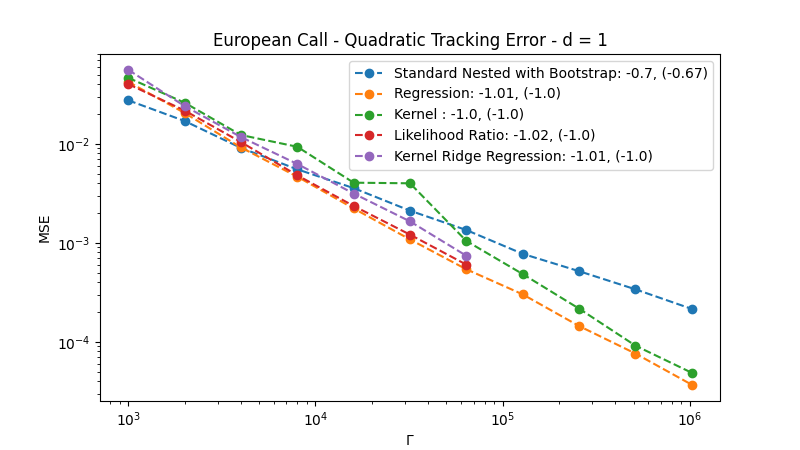
\includegraphics[width=0.7\textwidth]{./project1/figures/figure1.png}
    \caption{Empirical convergence of nested simulation procedures for quadratic tracking error on Portfolio 1 with $d=1$}
\label{fig1:compareAll} 
\end{figure}
In Figure~\ref{fig1:compareAll}, the \gls{mse}s of the nested simulation procedures are plotted against the total simulation budget $\Gamma$ in a log-log scale, where each point represents the average \gls{mse} of the corresponding estimator over \num{1000} macro replications of the same experiment.
Due to the difficulty of fixing $\Gamma$ for the \gls{mlmc} procedure, the empirical rate of convergence of the \gls{mlmc} procedure is not reported here, but a detailed analysis of the empirical convergence of the \gls{mlmc} procedure is provided in Section~\ref{sec1:empirical-mlmc}.

A regression line is fitted to the \gls{mse}s of each nested simulation procedure against the simulation budget $\Gamma$ in a log-log scale, and the slope of the fitted line is reported.
The slopes of the fitted lines can be interpreted as the empirical rates of convergence.
Alongside in the parentheses are the asymptotic rates of convergence obtained by the theoretical analysis in Section~\ref{sec1:asymptotic-convergence}.
By comparing the empirical rates of convergence with the asymptotic rates, we can observe how well the empirical rates of convergence match their asymptotic rates.
In the case illustrated in Figure~\ref{fig1:compareAll}, the empirical rates of all procedures closely match their asymptotic rates.

Except for the standard nested simulation procedure, the empirical rates of convergence of the other procedures are close to $\Gamma^{-1}$, i.e., all of them achieve similar finite-sample performance that is better than the standard procedure.
Pooling of inner simulation samples across different outer scenarios is the key reason behind their higher empirical rates of convergence.
However, pooling also introduces additional computational cost that is not reflected in the simulation budget $\Gamma$.
Due to the computational complexity of the likelihood ratio-based and the \gls{krr}-based procedures, their \gls{mse}s are not reported for $\Gamma$ larger than $\num{16000}$ and $\num{64000}$, respectively.
Detailed discussion of the additional computational cost of pooling is provided in Section~\ref{sec1:computational-complexity}.

In the following sections, we examine the empirical convergence of the nested simulation procedures similarly as in Figure~\ref{fig1:compareAll}.
With a more detailed analysis of different risk measures, option types, and asset dimensions, we aim at providing a comprehensive understanding and comparison of the convergence behavior of the nested simulation procedures in practice.

\subsection{Sensitivity to the Asset Dimension}\label{sec1:sensitivity-dimension}
In portfolio risk management, the asset dimension is a critical factor that determines the complexity of the portfolio and the computational cost of the risk measure estimation.
The theoretical analyses in Section~\ref{sec1:convergence-orders} suggest that the asymptotic rate of convergence of the nested simulation procedures, except for the kernel smoothing-based procedure, is independent of the asset dimension.
However, in practice, their empirical convergence behavior could be different.
In this section, we examine the sensitivity to the asset dimension of the empirical convergence of the nested simulation procedures.

\begin{figure}[ht!]
    \centering
    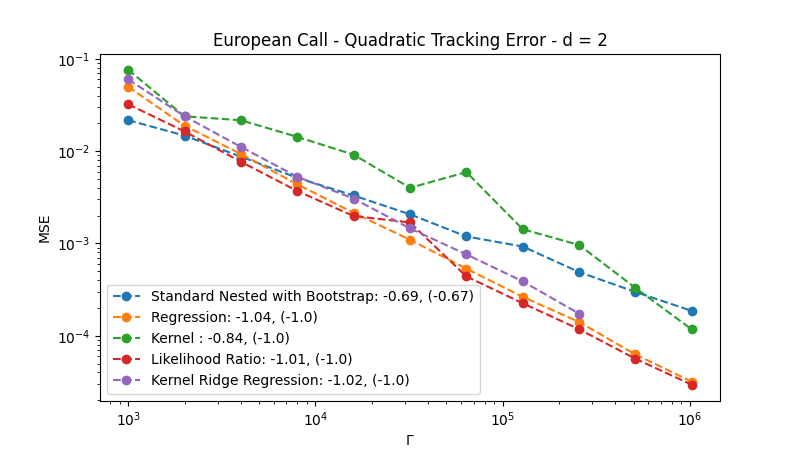
\includegraphics[width=0.48\textwidth]{./project1/figures/figure2a.png}
    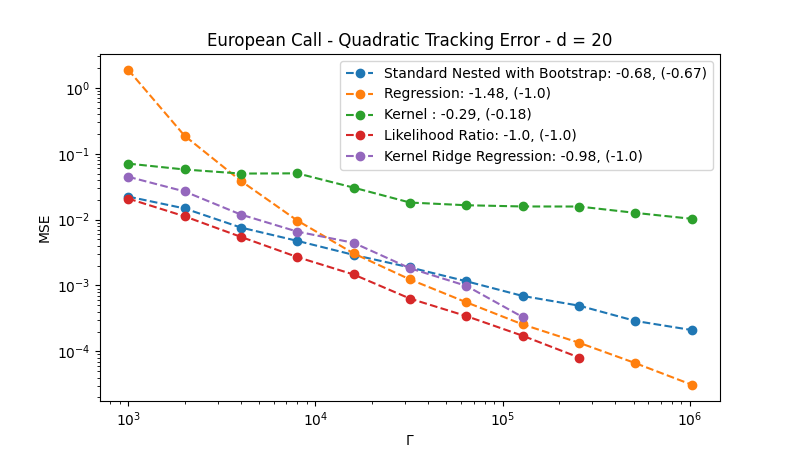
\includegraphics[width=0.48\textwidth]{./project1/figures/figure2b.png}
    \caption{Empirical convergence of nested simulation procedures for quadratic tracking error on Portfolio 1 with different asset dimensions}
\label{fig1:assetDimension} 
\end{figure}

In Figure~\ref{fig1:assetDimension}, the empirical convergence of the nested simulation procedures for a quadratic tracking error on Portfolio 1 is illustrated for different asset dimensions, i.e., $d = 2$ and $d = 20$.
The empirical rates of convergence of the standard, the \gls{krr}-based, and the likelihood ratio-based procedures closely match their asymptotic rates for both asset dimensions, and they are insensitive to an increase in the asset dimension.
In contrast, both the kernel smoothing-based and regression-based procedures are greatly affected by the asset dimension.
Their sensitivities to the asset dimension differ in finite-sample experiments:
\begin{itemize}    
    \item For the kernel smoothing-based procedure, the empirical rate of convergence decreases as the asset dimension increases. 
    This observation aligns with the theoretical analysis in Section~\ref{sec1:asymptotic-convergence}, which demonstrates that the asymptotic rate of convergence of the kernel smoothing-based procedure is sensitive to the asset dimension.
    Nevertheless, even for $d = 2$ and $d = 20$, the empirical rate remains higher than its asymptotic rate.
    \item For the regression-based procedure, the asymptotic rate is not affected by the asset dimension, but the empirical rates of convergence are higher than the asymptotic rates for both asset dimensions, and the empirical rate is higher for $d = 20$ than for $d = 2$.
\end{itemize}
In the following sections, we provide detailed explanations for the discrepancy between their empirical rates of convergence and their asymptotic rates.

\subsection{Empirical Convergence of Kernel Smoothing-Based Procedures}\label{sec1:kernel-smoothing-convergence}

Kernel smoothing is a non-parametric regression metamodel.
According to the theoretical analysis in Section~\ref{sec1:asymptotic-convergence}, the asymptotic rate of convergence of the kernel smoothing-based nested simulation procedure is highly dependent on the asset dimension $d$.
In this section, we use a \gls{knn} metamodel for the kernel smoothing-based nested simulation procedure, and we examine its empirical convergence for different asset dimensions.

\begin{figure}[ht!]
    \centering
    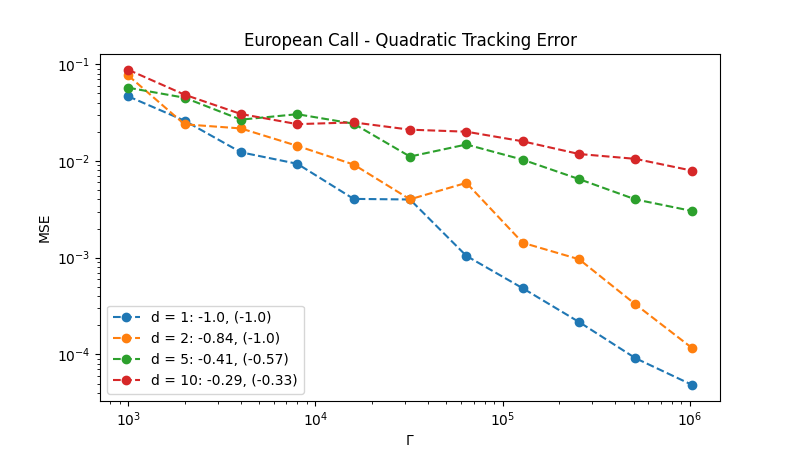
\includegraphics[width=0.48\textwidth]{./project1/figures/figure4a.png}
    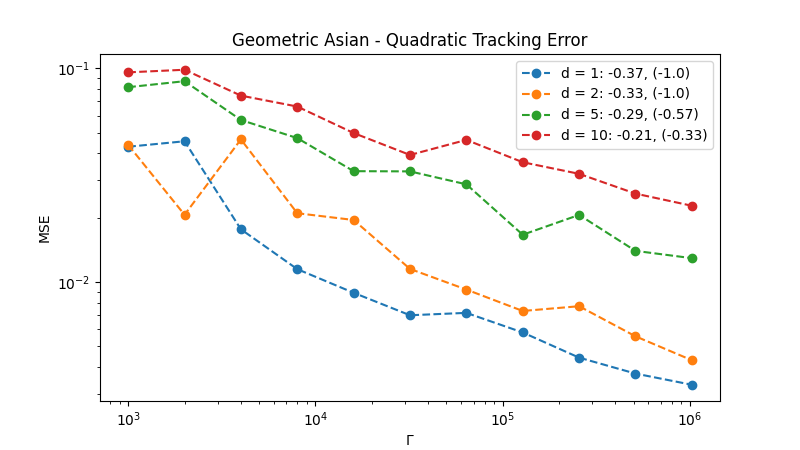
\includegraphics[width=0.48\textwidth]{./project1/figures/figure4b.png}
    \caption{Empirical convergence of kernel smoothing procedure for different values of $d$}
\label{fig1:kernel_d} 
\end{figure}

In Figure~\ref{fig1:kernel_d}, the empirical convergence of the kernel smoothing-based nested simulation procedure for a quadratic tracking error is illustrated for different asset dimensions, i.e., $d = 1, 2, 5, 10$.
The experiment finds that the kernel smoothing-based nested simulation procedure is extremely sensitive to the asset dimension and the payoff structure.
While the asset dimension is expected to be a critical factor as shown in the theoretical analysis, the payoff structure is an unexpected factor that affects the empirical convergence of the kernel smoothing-based nested simulation procedure.
For a portfolio with geometric Asian options, the payoff complexity is higher than that of a portfolio with European call options.
The empirical rate of convergence of the kernel smoothing-based procedure is substantially lower for the portfolio with geometric Asian options than for the portfolio with European call options.
For geometric Asian options, the empirical rates of convergence are even lower than the asymptotic rates for all asset dimensions.

Due to the computational cost of the kernel smoothing-based nested simulation procedure, we are not able to conduct experiments for higher budget levels.
However, we are able to conduct additional experiments to examine the effects of cross-validation on the empirical convergence of the kernel smoothing-based procedure.
Another phenomenon that is observed in Figure~\ref{fig1:kernel_d} is that the empirical rate of convergence of the kernel smoothing-based procedure does not decrease monotonically as the simulation budget increases.
This is likely due to the fact that the kernel smoothing-based procedure, as a non-parametric regression procedure, is highly dependent on the cross-validation of the hyperparameters of the metamodel.
For the kernel smoothing-based procedure, the \gls{knn} metamodel is implemented. 
Hence, the hyperparameter of interest is the number of nearest neighbors $k$.
In our numerical experiment, cross-validation is conducted once to select the optimal value of $k$ for each simulation budget, and the selected value of $k$ is fixed for all $\num{1000}$ replications.
Therefore, a suboptimal selection of the optimal value of $k$ can lead to a poor metamodel estimate, and the \gls{mse} of the kRR-based procedure will be dominated by the model error of the metamodel.

\begin{figure}[ht!]
    \centering
    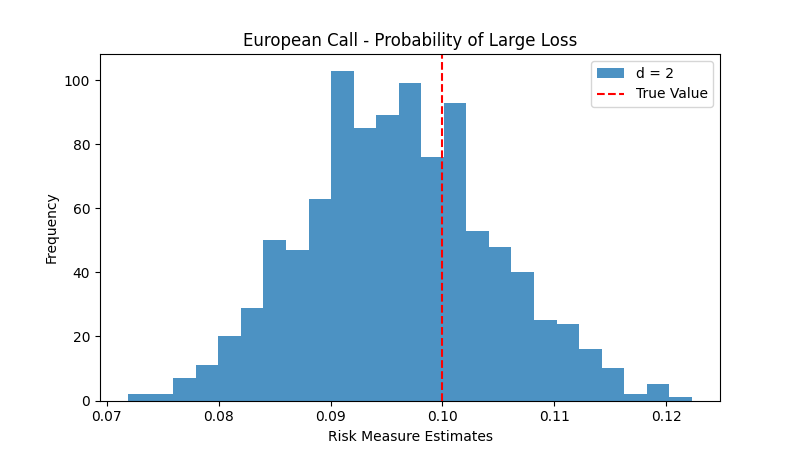
\includegraphics[width=0.48\textwidth]{./project1/figures/figure5a.png}
    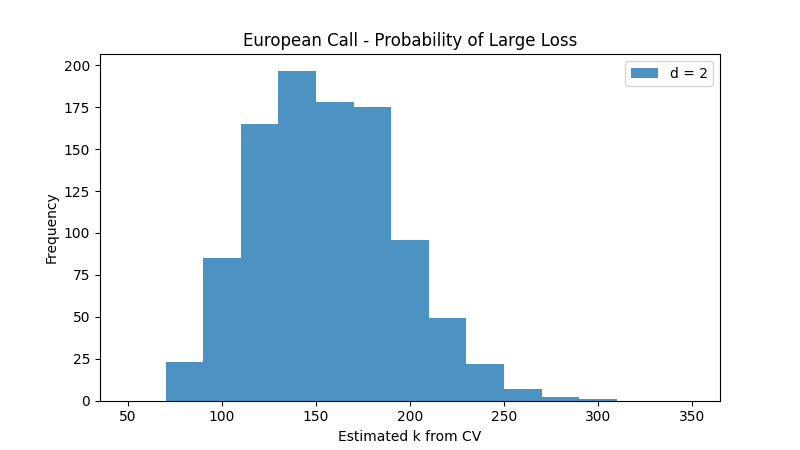
\includegraphics[width=0.48\textwidth]{./project1/figures/figure5b.png}
    \caption{Cross-validation for the kernel smoothing-based procedure with $\Gamma=\num{100000}$}
\label{fig1:kernel_cv} 
\end{figure}

In Figure~\ref{fig1:kernel_cv}, the empirical convergence of the kernel smoothing-based nested simulation procedure for the probability of large loss is illustrated for different values of $k$ with $\Gamma = \num{100000}$.
The observation is that the value of optimal $k$ estimated by cross-validation is highly variable across different replications.
For $d = 2$, the optimal value of $k$ is estimated to be between $120$ to $220$ for most replications, and the estimated risk measures are close to the true risk measure of $0.1$.
For the two replications where $k = 80$ is estimated as the optimal value of $k$, the resulting estimates of risk measures are $0.1187$ and $0.1189$, which are substantially higher than the estimated risk measures for the other replications and far from the true risk measure of $0.1$.
This observation suggests that the empirical convergence of the kernel smoothing-based nested simulation procedure is highly sensitive to the cross-validation of the hyperparameters of the metamodel.
A \gls{krr}-based nested simulation procedure suffers from the same problem. 
The fluctuation in Figure~\ref{fig1:kernel_d} is likely due to poor cross-validation of the hyperparameters of the metamodel.

\subsection{Empirical Convergence of Parametric Regression Procedures}\label{sec1:regression-convergence}

For both the regression-based and kernel smoothing-based procedures, the observed higher empirical rates of convergence can be explained by the poor performance of their metamodels at low simulation budgets. 
When simulation budgets are low, the metamodels trained to approximate the true inner simulation are inadequate.
The \gls{mse}s for these procedures are dominated by the model errors of the metamodels.
In other words, they have not yet reached their asymptotic convergence regimes.

Due to computation constraints, we are not able to conduct experiments for kernel smoothing-based nested simulation procedures for higher budget levels, but we are able to conduct additional experiments for the regression-based nested simulation procedure.
In our previous numerical experiments, the empirical rate of convergence of the regression procedure is observed to be much larger than its asymptotic rate of convergence.
For dimensions larger than $10$, the \gls{mse} of the regression procedure decreases quickly in the beginning, and its rate of decrease stabilizes after a certain budget level.
In Figure~\ref{fig1:reg_lb} illustrates the empirical convergence of the regression-based procedure in more detail at higher simulation budgets, where the asymptotic level of convergence is reached for $d = 20$.

\begin{figure}[ht]
    \centering
    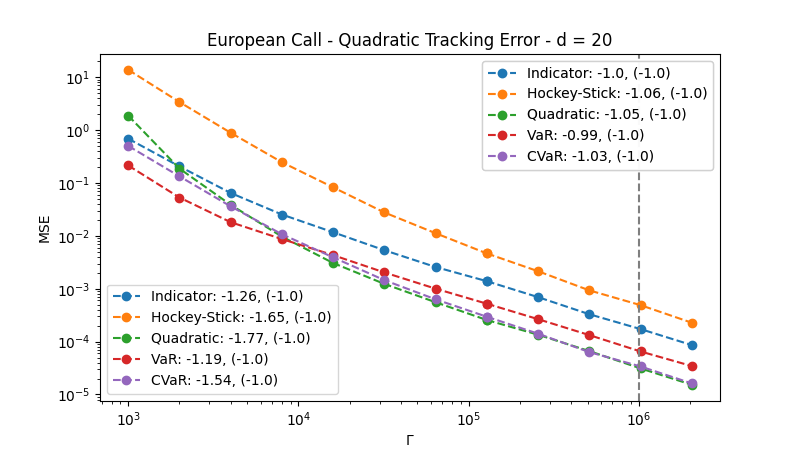
\includegraphics[width=0.7\textwidth]{./project1/figures/figure3.png}
    \caption{Empirical convergence of regression procedure for European call options and $d=20$}
\label{fig1:reg_lb} 
\end{figure}

The left part of Figure \ref{fig1:reg_lb} contains the \gls{mse}s of the regression procedure for budget sizes that are smaller than $10^3$. 
Slopes of the fitted lines on the left correspond to the empirical rate of convergence of the regression procedure for budget levels between $10^3$ and $10^4$.
To investigate the convergence behavior for higher budget levels, we conduct additional experiments for the European call option with a dimension of $20$. 
The additional experiments are summarized on the right side of Figure \ref{fig1:reg_lb}.
After reaching a certain budget level, i.e., $\Gamma = 10^6$ in our case, the empirical rate of convergence for the regression-based nested simulation procedure approaches its asymptotic rate. 
For nested simulation procedures with a biased metamodel, the metamodel estimates of the true inner simulation are poor, especially for smaller budget sizes. 
We are able to clearly observe this phenomenon for the regression metamodel, and it can be explained by dividing the \gls{mse} into metamodeling bias and simulation variance.
\begin{itemize}
    \item For small budget sizes, the improvement in the bias of the regression metamodel dominates the improvement in the simulation variance. 
    Performing poorly for extremely low simulation budgets, the regression metamodel improves dramatically as the simulation budget increases.
    \item As the simulation budget gets higher, the improvement of the regression bias becomes negligible compared with that of the simulation variance. 
    The regression metamodel ceases to improve after reaching a certain level ($\Gamma = 10^6$ in our case), and the improvement of simulation variance dominates.
\end{itemize}
Due to high computational costs, we are not able to conduct experiments for higher budget levels, but we expect the \gls{mse} of the regression-based nested simulation procedure to stabilize after $\Gamma = 10^6$, and the empirical rate of convergence to approach its asymptotic rate.
The empirical convergence rates reported in the graph legends are higher than the actual rates after regression-based nested simulation procedure reaches the asymptotic convergence regime.
In the context of nested simulation procedures, a parametric regression metamodel has several advantages over a non-parametric regression metamodel.
\begin{itemize}
    \item Parametric regression achieves a good empirical convergence behavior for a moderate simulation budget.
    \item Parametric regression is insensitive to changes in the asset dimension.
    \item Parametric regression is easier to implement.
    It does not require cross-validation to select the hyperparameters of the metamodel.
\end{itemize}
However, parametric regression suffers from the model misspecification risk.
More specifically, selecting a wrong regression basis can lead to a poor metamodel estimate, where the \gls{mse} of the nested simulation procedure is dominated by the model error of the metamodel~\citep{broadie2015risk}.

In our previous numerical experiments, the regression-based nested simulation procedure is implemented with Laguerre polynomials up to degree $3$ as the basis functions.
It is a standard choice in the literature.
To examine the sensitivity of the empirical convergence behavior to the regression basis, we consider different basis functions, i.e., regular polynomial regression up to degree $3$.

\begin{figure}[ht!] 
    \centering
    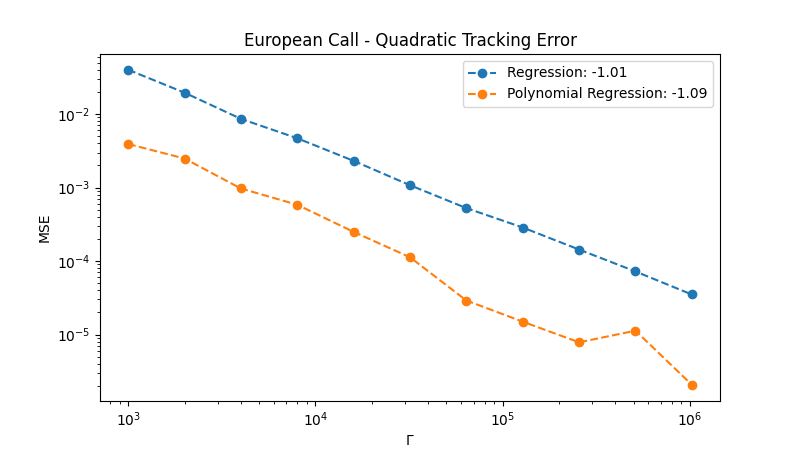
\includegraphics[width=0.48\textwidth]{./project1/figures/figure13a.png}
    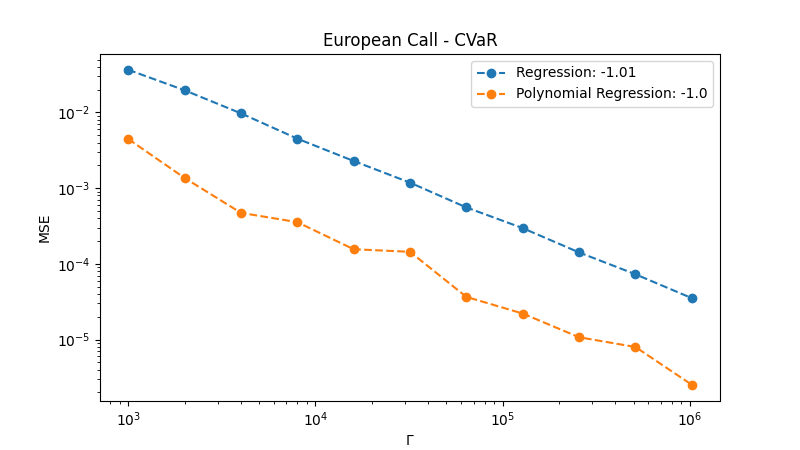
\includegraphics[width=0.48\textwidth]{./project1/figures/figure13b.png}
    \caption{Empirical convergence of regression-based nested simulation procedures for different regression bases}
\label{fig1:sens_basis}
\end{figure}

In Figure~\ref{fig1:sens_basis}, the empirical convergence results of the regression-based nested simulation procedure for a quadratic tracking error and a 90\%-\gls{cvar} are illustrated for the two different regression bases.
The empirical rates of convergence of the regression-based nested simulation procedure are observed to be insensitive to the chosen type of regression basis.

\subsection{Sensitivity to the Option Types and Risk Measures}\label{sec1:sensitivity-option-type}

In our previous numerical experiments, we have examined the empirical convergence behavior of the nested simulation procedures for European call options, which only depends on the asset price at maturity.
To examine the sensitivity of the empirical convergence behavior to the option type, we consider path-dependent options, which are geometric Asian options and barrier options.

\begin{figure}[ht!] 
    \centering
    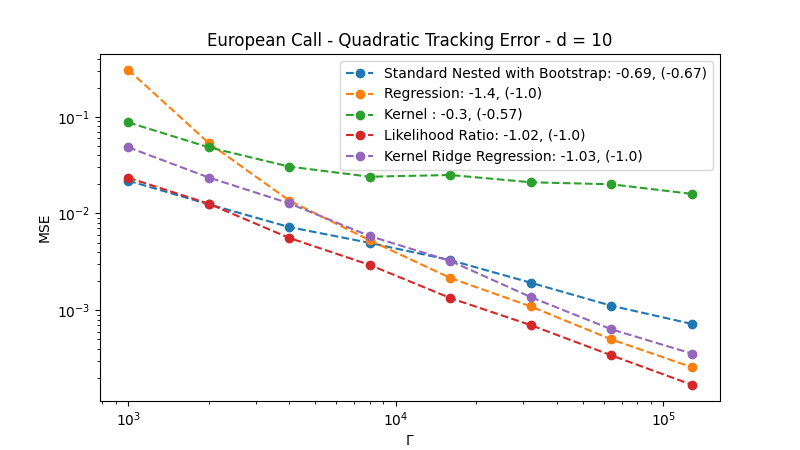
\includegraphics[width=0.48\textwidth]{./project1/figures/figure6a.png}
    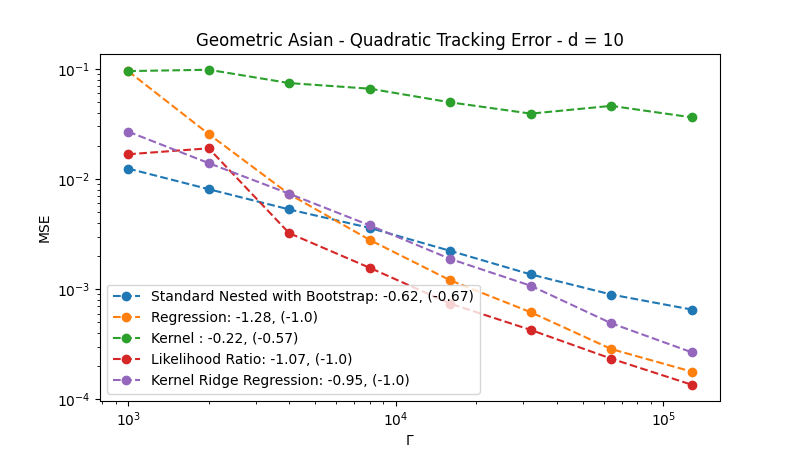
\includegraphics[width=0.48\textwidth]{./project1/figures/figure6b.png}
    \caption{Empirical convergence of nested simulation procedures for quadratic tracking error on different portfolios with $d=20$}
\label{fig1:1x03} 
\end{figure}

In Figure~\ref{fig1:1x03}, the empirical convergence of the nested simulation procedures for the quadratic tracking errors of Portfolio 1 and Portfolio 4 is illustrated for $d = 20$.
The empirical rates of standard, likelihood ratio-based, and \gls{krr}-based nested simulation procedures closely ensemble their asymptotic rates for path-dependent options.
The empirical rate of convergence of the regression-based and kernel smoothing-based procedures is much higher than their asymptotic rates for barrier options. 
The reasons are explained in Section~\ref{sec1:regression-convergence} and Section~\ref{sec1:kernel-smoothing-convergence}.

\begin{figure}[ht!] 
    \centering
    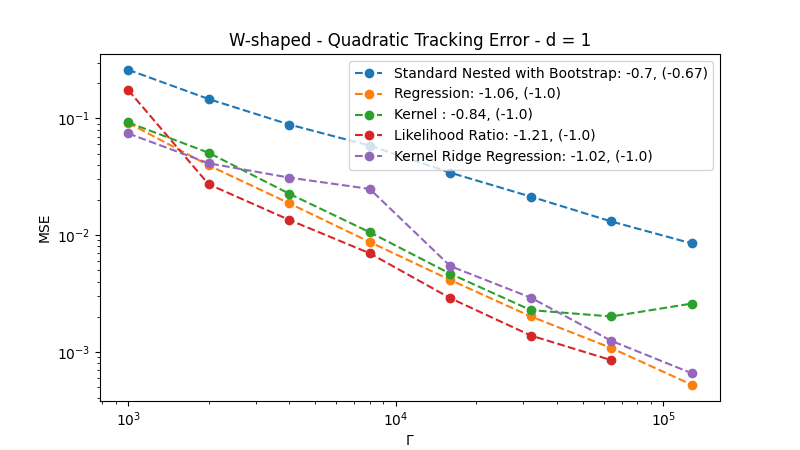
\includegraphics[width=0.48\textwidth]{./project1/figures/figure7a.png}
    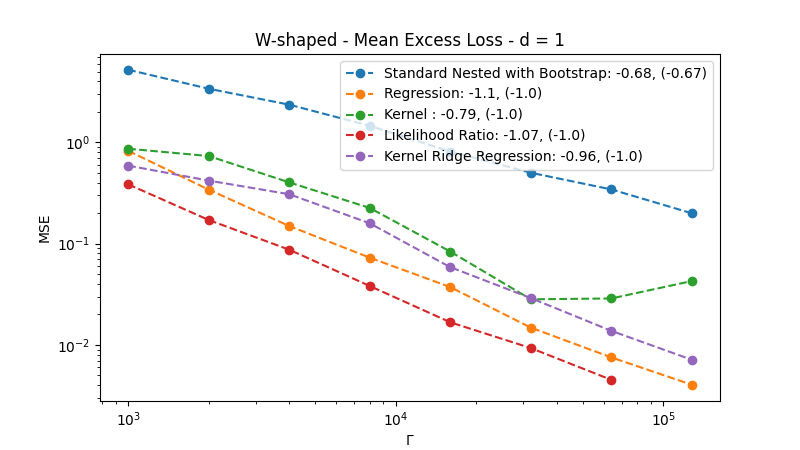
\includegraphics[width=0.48\textwidth]{./project1/figures/figure7b.png}
    \caption{Empirical convergence of nested simulation procedures for a W-shaped payoff}
\label{fig1:5503} 
\end{figure}

In~\cite{broadie2015risk}, the authors propose a numerical example where the payoff has a W-shape with respect to the asset price at maturity.
We have incorporated this example as Portfolio 5.
In Figure~\ref{fig1:5503}, the empirical convergence of the nested simulation procedures for a quadratic tracking error and a mean excess loss on Portfolio 5 is illustrated for $d = 1$.
For all procedures, we observe a similar convergence behavior as in other path-dependent options.
The \gls{mse}s of the kernel smoothing-based and \gls{krr}-based procedures do not decrease monotonically as the simulation budget increases.
This fluctuating behavior is observed and analyzed in Section~\ref{sec1:kernel-smoothing-convergence}.

\begin{figure}[ht!] 
    \centering
    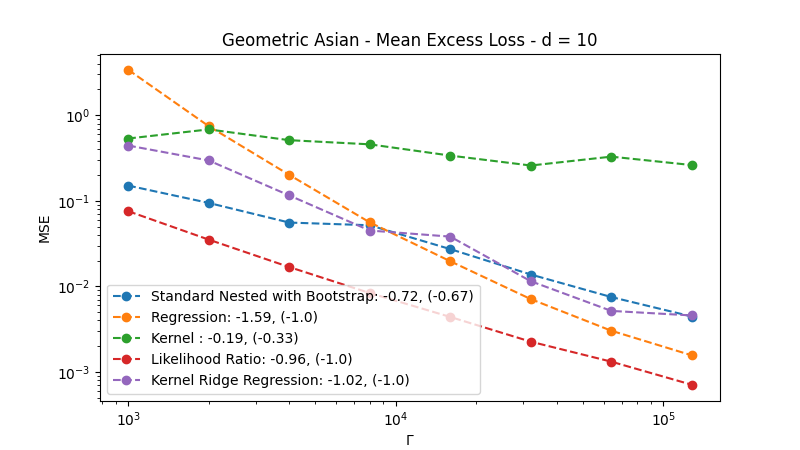
\includegraphics[width=0.48\textwidth]{./project1/figures/figure8a.png}
    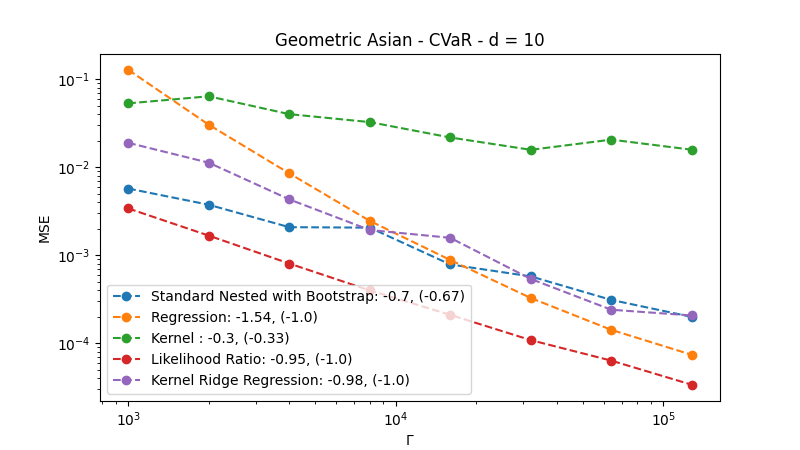
\includegraphics[width=0.48\textwidth]{./project1/figures/figure8b.png}
    \caption{Empirical convergence of nested simulation procedures for different risk measures on Portfolio 1 with $d=20$}
\label{fig1:110x}
\end{figure}

Figure~\ref{fig1:110x} illustrates similar observations for sensitivity to different risk measures.
A change in the risk measure of interest does not affect the empirical convergence behavior of all nested simulation procedures.
From the empirical convergence results, we observe that the empirical rates of convergence of the regression-based nested simulation procedure are the highest among all nested simulation procedures for all risk measures and option types.
Furthermore, the regression-based procedure is stable across different payoff structures and risk measures. 
Its \gls{mse}s decrease quickly in the beginning, and after reaching a certain level of $\Gamma$, the rate of decrease stabilizes to match its asymptotic rate of convergence.
Parametric regression is the most attractive metamodel for nested simulation procedures due to its fast empirical convergence behavior, stability across different payoff structures and risk measures, and ease of implementation.
The following sections focus on the regression-based nested simulation procedure for the rest of the numerical experiments.

\subsection{Sensitivity to level for VaR and CVaR}\label{sec1:sensitivity-level}

The level of \gls{var} and \gls{cvar} is a critical factor that determines the complexity of the risk measure estimation.
In our previous numerical experiments, the level of \gls{var} and \gls{cvar} is set to be the $90\%$ quantile of the distribution of the inner simulation noise.
In this section, we examine the empirical convergence of the regression-based nested simulation procedures for other levels of \gls{var} and \gls{cvar}, i.e., $80\%$, $95\%$, $99\%$, and $99.6\%$.

\begin{figure}[ht!] 
    \centering
    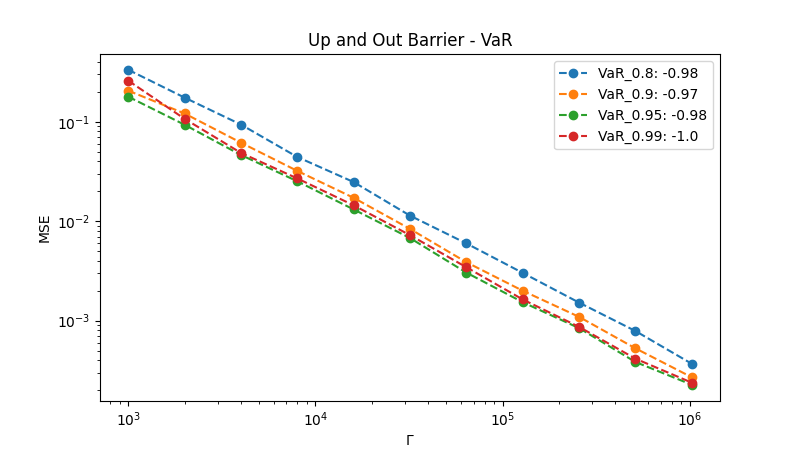
\includegraphics[width=0.48\textwidth]{./project1/figures/figure9a.png}
    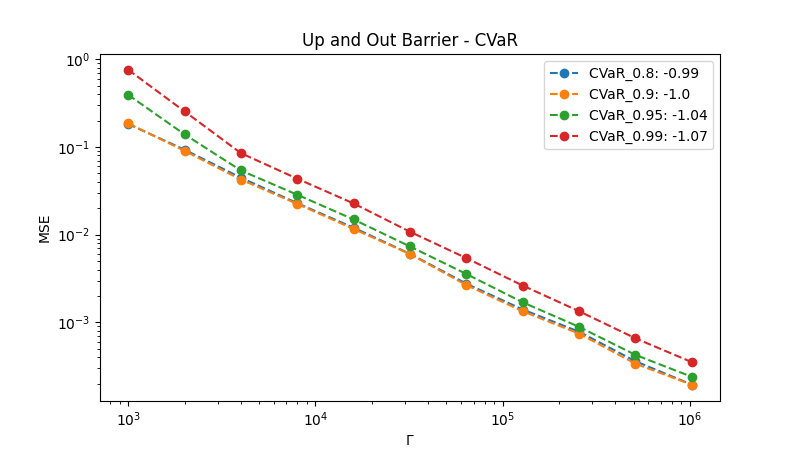
\includegraphics[width=0.48\textwidth]{./project1/figures/figure9b.png}
    \caption{Empirical convergence of regression-based procedures for different levels of VaR and CVaR for Up and Out Barrier Call Options}
\label{fig1:sens_level}
\end{figure}

In Figure~\ref{fig1:sens_level}, the empirical convergence of the regression-based nested simulation procedure for different levels of \gls{var} and \gls{cvar} is illustrated for up-and-out barrier call options.
The empirical rates of convergence of the regression-based nested simulation procedure are not sensitive to the level of \gls{var} and \gls{cvar}.

\subsection{Sensitivity to the Asset Model}\label{sec1:sensitivity-assetModel}

Our previous numerical experiments have been conducted under the assumption that the underlying asset dynamics follow a multidimensional \gls{gbm} with $0.3$ pairwise correlation.
To examine the sensitivity of the empirical convergence behavior to the asset model, we consider a stochastic volatility model of a Heston type~\citep{heston1993closed}.
In a Heston model, the asset price and the volatility are correlated, and the volatility is a stochastic process.

\begin{align*}
    dS_t &= \mu S_t dt + \sqrt{v_t} S_t dW_{1,t}, \\
    dv_t &= \kappa (\theta - v_t) dt + \xi \sqrt{v_t} dW_{2,t},
\end{align*}
where $W_{1,t}$ and $W_{2,t}$ are two independent Brownian motions.

In this experiment, the initial asset price and the volatility are set to be $100$ and $0.2$, respectively. The parameters are set to be $\mu = 0.08$, $\kappa = 2$, $\theta = 0.04$, $\xi = 0.1$.

\begin{figure}[ht!] 
    \centering
    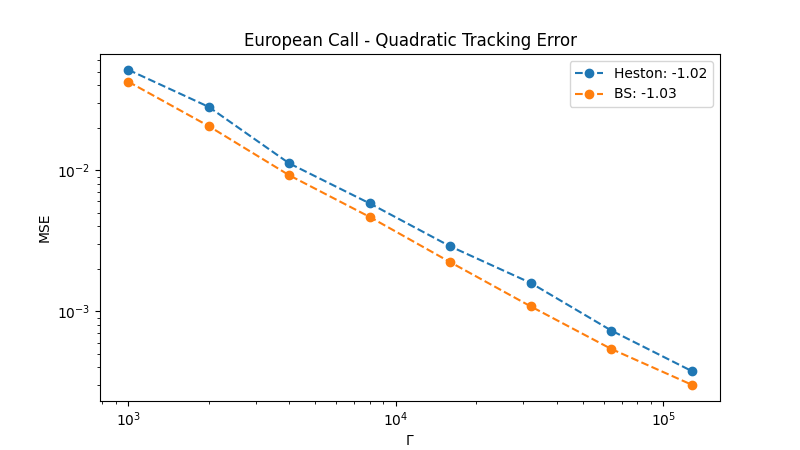
\includegraphics[width=0.48\textwidth]{./project1/figures/figure10a.png}
    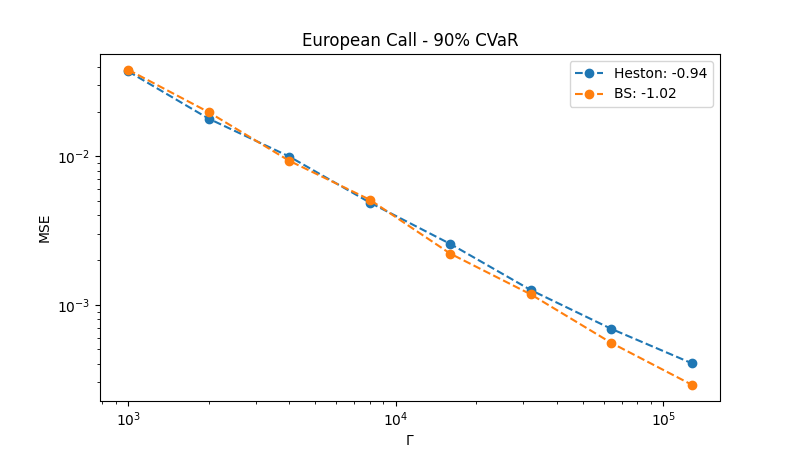
\includegraphics[width=0.48\textwidth]{./project1/figures/figure10b.png}
    \caption{Empirical convergence of regression-based nested simulation procedures for different asset models}
\label{fig1:sens_model}
\end{figure}

In Figure~\ref{fig1:sens_model}, the empirical convergence results of the regression-based nested simulation procedure for a quadratic tracking error and a 90\%-\gls{cvar} are illustrated for different asset models, i.e., a \gls{gbm} and a Heston model.
The empirical rates of convergence of the regression-based nested simulation procedure are observed to be insensitive to the asset model.

In summary, we find the empirical convergence behavior of the regression-based nested simulation procedure to be stable across different risk measures, option types, asset dimensions, levels of \gls{var} and \gls{cvar}, asset models, and regression bases.
With a limited total budget, the regression-based nested simulation procedure is the most robust and stable among all nested simulation procedures. 

\subsection{Empirical Convergence of MLMC}\label{sec1:empirical-mlmc}

The \gls{mlmc} procedure is a variance reduction technique that is designed to reduce the computational cost of nested simulation procedures.
The theoretical analysis in~\cite{giles2019multilevel} shows that the \gls{mlmc} procedure has a faster empirical rate of convergence than the standard nested simulation procedure when the risk measure of interest is the probability of a large loss over a threshold $u$, i.e., the nested expectation case with $h$ being an indicator function.
In this numerical experiment, the initial number of inner replications, the refinement factor, the r-value for adaptive algorithm are set to be $4$, $4$, and $1.5$, respectively.
We note that the \gls{mlmc} procedure focuses on adaptive allocation of the simulation budget and is fundamentally different from supervised learning-based nested simulation procedures. And their results are not directly comparable.

\begin{table}[ht]
    \centering
    \begin{tabular}{rrrrrr}
    \toprule
    \textbf{Level} & \textbf{Bias} & \textbf{Variance} & \textbf{\gls{mse}} & $\Gamma$ & \textbf{\gls{mse} of SNS} \\ 
    \hline\hline
    0 & 0.118  & 0.104  & 0.1364 & 6400     & 0.1660    \\
    1 & 0.102  & 0.0916 & 0.1020 & 27600    & 0.1305    \\
    2 & 0.0870 & 0.0794 & 0.0870 & 76600    & 0.0954    \\
    3 & 0.0815 & 0.0746 & 0.0812 & 175600   & 0.0744    \\
    4 & 0.0893 & 0.0805 & 0.0884 & 348100   & 0.0460    \\
    5 & 0.0750 & 0.0694 & 0.0750 & 640000   & 0.0366    \\
    \bottomrule
    \end{tabular}
    \caption{MSEs of the MLMC procedure for different levels}
\label{tab1:mlmc-mse}
\end{table}

We provide a summary of the empirical convergence results of the \gls{mlmc} procedure with a decomposition table of the \gls{mse}s in Table~\ref{tab1:mlmc-mse}.
The \gls{mse}s of the \gls{mlmc} procedure are decomposed into the bias and the variance of the estimator.
The \gls{mse}s of the standard nested simulation procedure with a similar total simulation budget are also provided for comparison.
Since the \gls{mlmc} procedure is designed with a fixed number of outer simulation paths, the benefit of the \gls{mlmc} procedure is minimal when the total simulation budget is large.
More specifically, when $\Gamma$ is large, the standard nested simulation procedure with a bootstrap-based budget allocation strategy benefits from having a larger number of outer simulation paths, and the \gls{mse} of the standard nested simulation procedure is lower than that of the \gls{mlmc} procedure with a fixed number of outer simulation paths.

\section{Computational Complexity}\label{sec1:computational-complexity}
Compared to the standard procedure, metamodel-based nested simulation procedures often have faster empirical rates of convergence.
Their faster convergence benefits from the pooling of inner samples through the metamodels. 
However, pooling itself comes with increased computational costs, which are usually ignored in most numerical comparisons. 
This section summarizes the algorithmic complexity and illustrate the computational time of different nested simulation procedures.
The findings can provide some further guidance on the choice of a proper nested simulation procedure given a nested estimation problem.
Define basic operations to be basic mathematical operators, that is, arithmetic with individual elements has complexity $\mathcal{O}(1)$.

\begin{table}[ht]
    \centering  
    \small
    \begin{tabular}{llll}
    \hline
    \textbf{Procedures}      & \textbf{Training cost}                    &  \textbf{Prediction cost}    & \textbf{Total additional cost} \\ \hline \hline
    Standard procedure       &  $0$                                      &  $\mathcal{O}(M)$            & $\mathcal{O}(M)$ \\ 
    Regression               &  $\mathcal{O}(p^2M) + \mathcal{O}(p^3)$   &  $\mathcal{O}(pM)$           & $\mathcal{O}(p^2M) + \mathcal{O}(p^3)$ \\
    Kernel smoothing         &  $\mathcal{O}(M\log(M))$                  &  $\mathcal{O}(k\log(M))$     & $\mathcal{O}(M\log(M))$ \\
    Kernel ridge regression  &  $\mathcal{O}(M^3)$                       &  $\mathcal{O}(M^2)$          & $\mathcal{O}(M^3)$ \\
    Likelihood ratio         &  $0$                                      &  $\mathcal{O}(M^2)$          & $\mathcal{O}(M^2)$ \\
    \hline
    \end{tabular} 
    \caption{Additional computational costs of nested simulation procedures aside from simulation}
\label{tab1:complexity}
\end{table}

Table~\ref{tab1:complexity} shows the algorithmic complexity of the nested simulation procedures.
For a $d$-dimensional nested estimation problem, the simulation cost for all procedures is $\mathcal{O}(dMN)$.
The simulation cost is omitted from Table~\ref{tab1:complexity}, as all procedures are given the same simulation budget.
Given $M$ outer samples and the corresponding $M$ inner sample averages, the algorithmic complexity of the additional operations does not involve $N$ and thus, can be written in terms of $M$ only. 
The training cost includes the cost of fitting the metamodel and the cost of cross-validation for non-parametric regression metamodels.

For the standard procedure, 
\begin{itemize}
    \item the training cost is $0$ due to the absence of a metamodel. 
    \item Its prediction cost $\mathcal{O}(M)$ comes from the evaluation of the function $h$ for $M$ samples.
\end{itemize}
For the regression-based procedure, a linear regression model is fitted with $p$ predictors.
\begin{itemize}
    \item The training cost is $\mathcal{O}(p^2M) + \mathcal{O}(p^3)$.
          Estimating the coefficients of the regression model involves multiplying the design matrix by its transpose and inverting the resulting matrix, which has complexity $\mathcal{O}(p^2M)$ and $\mathcal{O}(p^3)$, respectively.
          For a review in the complexity of a matrix inversion, see~\cite{stothers2010complexity}.
          The matrix inversion has complexity $\mathcal{O}(p^3)$ using a Gauss-Jordan elimination, but in practice, the complexity can be reduced to $\mathcal{O}(p^{2.807})$ by~\cite{strassen1969gaussian} and $\mathcal{O}(p^{2.376})$ by~\cite{coppersmith1987matrix}.
          In practice, $p$ is usually much smaller than $M$ and does not grow with the simulation budget $\Gamma$.
          $p$ is fixed by the basis function, which is selected based on the complexity of the payoff function.
    \item The prediction cost of the regression-based procedure is $\mathcal{O}(pM)$, which comes from the multiplication of the design matrix by the estimated coefficients.
\end{itemize}
For the kernel smoothing-based procedure, the \gls{knn} metamodel is implemented. 
In practice, the K-D tree algorithm~\citep{bentley1975multidimensional} is often implemented for an efficient nearest neighbor search.
\begin{itemize}
    \item During training, a tree is constructed to store the distance, which has a degree of complexity of $\mathcal{O}(M\log(M))$.
    \item The prediction cost of the kernel smoothing-based procedure is $\mathcal{O}(kM\log(M))$, which comes from a query of the K-D tree for $k$ nearest neighbors for $M$ samples.
    Conversely, an inefficient algorithm calculates the distance matrix during training and a block sort algorithm to find the $k$ nearest neighbors, which results in a degree of complexity of $\mathcal{O}(M^2)$ and $\mathcal{O}(M^2\log(M))$, respectively.
    A practical implementation of a block sort is provided in~\cite{kim2008ratio}.
    Hence, an efficient implementation of the \gls{knn} metamodel is crucial for the kernel smoothing-based procedure.
\end{itemize}
For the likelihood ratio-based procedure, 
\begin{itemize}
    \item the training cost is $0$ as no training is required.
    \item The prediction cost of the likelihood ratio-based procedure is $\mathcal{O}(M^2)$, which comes from the calculation of the likelihood weights for $M$ samples.
\end{itemize}
For the \gls{krr}-based procedure, 
\begin{itemize}
    \item the main training cost comes from inverting an $M \times M$ kernel matrix~\citep{scholkopf2002learning}, which has a degree of complexity of $\mathcal{O}(M^3)$ using a Gauss-Jordan elimination.
          Similar to the regression-based procedure, this complexity can be reduced to $\mathcal{O}(M^{2.376})$.
    \item The prediction cost of the \gls{krr}-based procedure is $\mathcal{O}(M^2)$, which comes from the multiplication of the kernel matrix by the estimated coefficients.
\end{itemize}
Among the metamodel-based procedures, parametric regression is the most efficient.
In the multiple linear regression, the number of features is usually much less than the number of data points, i.e., $p<M$. 
Kernel smoothing and \gls{var} are kernel-based metamodels, and they are more computaional expensive due to distance calculations and cross-validations of hyperparameters. 
The \gls{knn} metamodel has only 1 hyperparameter $k$, while the \gls{var} metamodel requires 3 hyperparameters, namely a smoothness hyperparameter $\nu$, a scale hyperparameter $\upsilon$, and a regularization hyperparameter $\lambda$.
Calculating the likelihood ratio weights is inevitable for the likelihood ratio-based procedure. 
While a k-fold cross-validation is used to estimate the hyperparameter for \gls{knn}, the \gls{var} requires Bayesian optimization~\citep{shahriari2015taking} to estimate the hyperparameters due to having a high-dimensional search space.
The likelihood ratio-based procedure requires no training, but the cost of calculating the likelihood weights is $\mathcal{O}(M^2)$.
Comparing the algorithmic complexity of the nested simulation procedures, the regression-based procedure is the most efficient among the metamodel-based procedures.
For a fixed $p$, the total additional cost of a regression-based procedure is $\mathcal{O}(M)$, which is the same as the standard procedure's.

\begin{figure}[ht!]
    \centering
    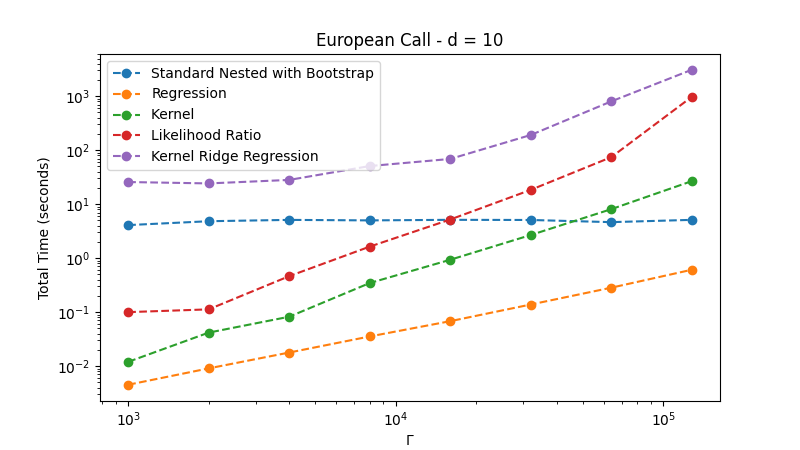
\includegraphics[width=0.48\textwidth]{./project1/figures/figure11a.png}
    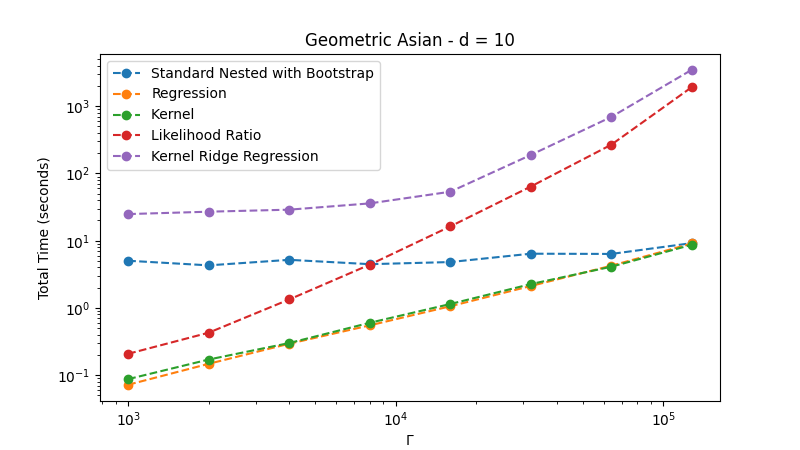
\includegraphics[width=0.48\textwidth]{./project1/figures/figure11b.png}
    \caption{Total computational cost for different procedures with $d=10$}
\label{fig1:tcc}
\end{figure}

The cost associated with pooling makes a major impact on the overall computational complexity of a metamodel-based nested simulation procedure.
In our finite-sample experiments, we have indeed observed that the actual computational cost to deviate substantially from the simulation cost.
In Figure~\ref{fig1:tcc}, the total actual computational time of different nested simulation procedures for European call options and geometric Asian options with $d = 10$ is illustrated in a log-log scale.
The $x$-axis shows the total simulation budget $\Gamma$, and the $y$-axis is the total computational time for 1 replication of the numerical experiment, in seconds.
All procedures are implemented on a machine with an AMD Ryzen 9 7900X processor with 32 GB of RAM.
8 cores are used for parallel computing, and the total computational time is the sum of the simulation time, the training time, and the prediction time.
The regression and kernel smoothing-based procedures are the most efficient among the metamodel-based procedures.
Since the regression-based procedure has a higher empirical rate of convergence, it is preferred over \gls{knn}.
The likelihood ratio-based and \gls{krr}-based procedures are the most computationally expensive among all procedures.
They are also demanding in terms of memory.
For budgets larger than $10^5$, the likelihood ratio-based procedure becomes impractical as storage of the likelihood weights becomes a bottleneck.
The \gls{krr}-based procedure suffers from both cross-validation and inverting a kernel matrix of size $M \times M$.
To separate the total computational time into different attributes, we provide a detailed analysis of the total computational time in the remainder of this section.

\begin{figure}[ht!]
    \centering
    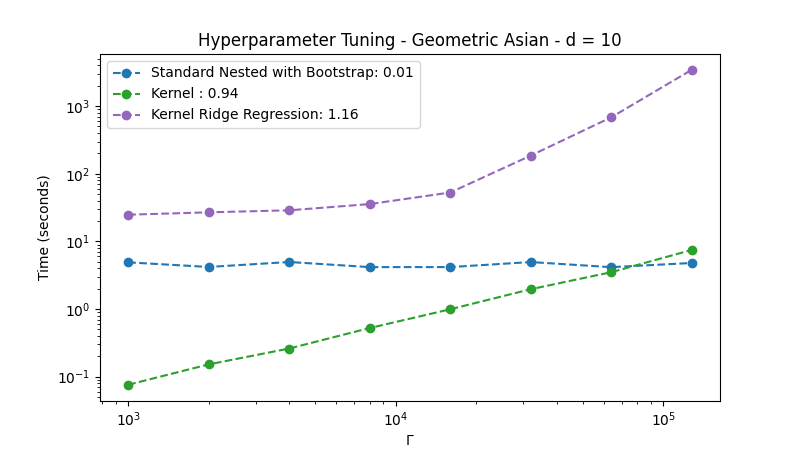
\includegraphics[width=0.48\textwidth]{./project1/figures/figure12a.png}
    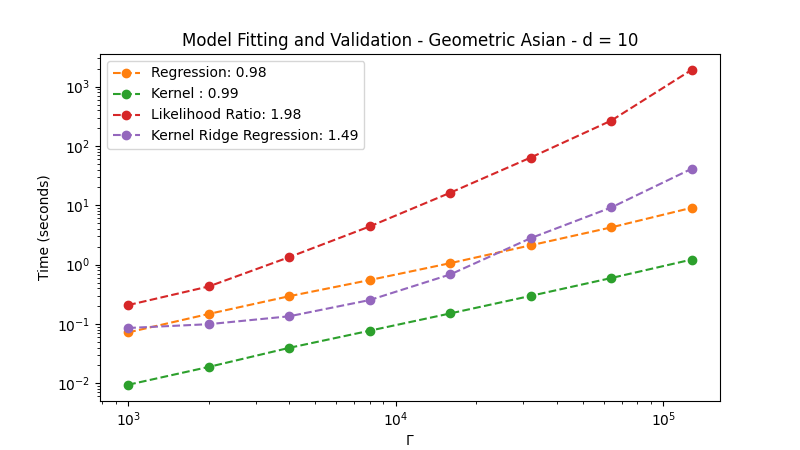
\includegraphics[width=0.48\textwidth]{./project1/figures/figure12b.png}
    \caption{Computational cost for implementing nested simulation procedures with $d=10$, excluding simulation time}
\label{fig1:c_model}
\end{figure}

Figure~\ref{fig1:c_model} illustrates the computational time of implementing different nested simulation procedures for the portfolio of geometric Asian options with $d = 10$.
The simulation time is omitted as it is the same for all procedures.
The remaining computations can be decomposed into two parts: hyperparameter tuning and model implementation.
The hyperparameter tuning cost is the cost of estimating the optimal hyperparameters for the metamodels, and the model implementation cost is the cost of fitting the metamodels and generating predictions from the trained metamodels.
For each procedure, each point in Figure~\ref{fig1:c_model} represents the average computational time for a given simulation budget $\Gamma$.
A regression model is fitted to each model respectively, and its slope can be viewed as the growth rate of the computational time with respect to $\Gamma$.
\begin{itemize}
    \item The total computational time of the standard procedure is mostly attributed to finding the optimal $M$ and $N$ using the bootstrap-based budget allocation strategy from~\cite{zhang2021bootstrap}.
    This cost does not grow with the simulation budget $\Gamma$, as its slope is close to $0$.
    \item The regression-based procedure does not require any hyperparameter tuning, and its total computational time is mainly attributed to the model implementation.
    The slope of the regression line is close to $1$, resembling its algorithmic complexity reported in Table~\ref{tab1:complexity}.
    \item The kernel smoothing-based and \gls{krr}-based procedure requires a cross-validation procedure to estimate the optimal hyperparameters. 
    In our implementation of \gls{knn}, the cross-validation is conducted by using a grid search with a search space which cardinality does not grow with the simulation budget $\Gamma$.
    However, the cross-validation cost of the kernel smoothing-based procedure grows with the simulation budget $\Gamma$ as more samples are involved.
    The \gls{krr}-based procedure requires a Bayesian optimization to estimate the optimal hyperparameters, and the cardinality of the search space also grows with the simulation budget $\Gamma$.
    The empirical cost of the \gls{krr}-based procedure does not resemble its algorithmic complexity reported in Table~\ref{tab1:complexity}.
    The efficient implementation of \gls{var} is an active area of research, and the computational cost of \gls{var} can be reduced by using a low-rank approximation of the kernel matrix, e.g., the Nystr\"om method~\citep{nystrom1930praktische}.
    Our observation for the \gls{var} implementation time is in line with the findings in~\cite{scikit-learn}, where the cost of \gls{var} is reported to be increasing quickly with the number of samples.
    \item The likelihood ratio-based procedure requires no hyperparameter tuning, and its total computational time is mainly attributed to the likelihood weight calculation, which is $\mathcal{O}(M^2)$. 
\end{itemize}
In summary, for a large simulation budget, the regression-based procedure is the most efficient among all metamodel-based procedures in terms of computational time.
For moderate simulation budgets, the regression-based procedure is a preferred choice.

\section{Conclusion and Extensions}\label{sec1:conclusion}
In the task of estimating risk measures for portfolios of complex financial derivatives, nested simulation procedures are commonly required but often computationally expensive. 
Tremendous efforts have been made to improve the efficiency of nested simulation procedures by approximating the inner simulation model with a metamodel. 
In this study, we review the literature on nested simulation procedures in financial engineering and provide fair comparisons of different metamodels by using the same set of numerical examples. 
Asymptotic properties of estimators for different nested simulation procedures are influenced by their corresponding metamodels.
To show an asymptotic convergence result, a more complex metamodels requires a more stringent set of assumptions on the distribution of the outer scenario and the inner simulation noise.
In terms of finite-sample behavior, this study provides a comprehensive comparison of different nested simulation procedures, and the findings can be used to guide the choice of a proper nested simulation procedure for a given nested estimation problem.
With extensive numerical experiments, we have found that the finite-sample performance of a procedure can deviate from its theory. 
In theory, supervised learning-based nested simulation procedures often provide higher rates of convergence, but they come at the computational expense of model training and generating predictions from the trained models. 
The likelihood ratio-based procedure requires no training, but it is expensive to compute, and it is also expensive to store the likelihood weights.
As a result, the total computational budget is not necessarily the same as the simulation budget, which is usually a limiting factor for practical applications.
A kernel-based procedure, e.g., \gls{knn} and \gls{var}, requires cross-validation, and its empirical performance depends heavily on the choice of hyperparameters.
A \gls{knn}-based procedure is sensitive to the asset dimension and the problem complexity.
A \gls{krr}-based procedure is computationally expensive, and its cost grows quickly with the simulation budget.
For kernel-based procedures, the computational cost is heavily dependent on the efficient implementation of the associated algorithms.
For a nested estimation problem with a given computational budget, we suggest the use of the regression-based simulation procedure when the budget size is moderate. 
It is efficient to implement, and it exhibits fast empirical convergence in estimating risk measures for popular option portfolios. 
However, we have only examined the performance for option portfolios in this study, where finding a suitable set of basis functions for regression is relatively easy.
In practice, a \gls{va} contract is often high-dimensional in time with a complex payoff structure, and it is a challenging problem for nested simulation procedures.
The time dependence in the feature space leads to multi-collinearity, and the regression-based procedure may not be the best choice in such instances.
In such cases, a neural network-based procedure may be more suitable, as it is a data-driven algorithm that finds a suitable set of basis functions automatically.
In Chapter~\ref{chap:project2}, we examine the performance of regression-based and neural network-based nested simulation procedures for estimating risk measures for \gls{va} contracts.
